% Options for packages loaded elsewhere
\PassOptionsToPackage{unicode}{hyperref}
\PassOptionsToPackage{hyphens}{url}
\PassOptionsToPackage{dvipsnames,svgnames,x11names}{xcolor}
%
\documentclass[
  number,
  review]{elsarticle}

\usepackage{amsmath,amssymb}
\usepackage{iftex}
\ifPDFTeX
  \usepackage[T1]{fontenc}
  \usepackage[utf8]{inputenc}
  \usepackage{textcomp} % provide euro and other symbols
\else % if luatex or xetex
  \usepackage{unicode-math}
  \defaultfontfeatures{Scale=MatchLowercase}
  \defaultfontfeatures[\rmfamily]{Ligatures=TeX,Scale=1}
\fi
\usepackage{lmodern}
\ifPDFTeX\else  
    % xetex/luatex font selection
\fi
% Use upquote if available, for straight quotes in verbatim environments
\IfFileExists{upquote.sty}{\usepackage{upquote}}{}
\IfFileExists{microtype.sty}{% use microtype if available
  \usepackage[]{microtype}
  \UseMicrotypeSet[protrusion]{basicmath} % disable protrusion for tt fonts
}{}
\makeatletter
\@ifundefined{KOMAClassName}{% if non-KOMA class
  \IfFileExists{parskip.sty}{%
    \usepackage{parskip}
  }{% else
    \setlength{\parindent}{0pt}
    \setlength{\parskip}{6pt plus 2pt minus 1pt}}
}{% if KOMA class
  \KOMAoptions{parskip=half}}
\makeatother
\usepackage{xcolor}
\setlength{\emergencystretch}{3em} % prevent overfull lines
\setcounter{secnumdepth}{5}
% Make \paragraph and \subparagraph free-standing
\makeatletter
\ifx\paragraph\undefined\else
  \let\oldparagraph\paragraph
  \renewcommand{\paragraph}{
    \@ifstar
      \xxxParagraphStar
      \xxxParagraphNoStar
  }
  \newcommand{\xxxParagraphStar}[1]{\oldparagraph*{#1}\mbox{}}
  \newcommand{\xxxParagraphNoStar}[1]{\oldparagraph{#1}\mbox{}}
\fi
\ifx\subparagraph\undefined\else
  \let\oldsubparagraph\subparagraph
  \renewcommand{\subparagraph}{
    \@ifstar
      \xxxSubParagraphStar
      \xxxSubParagraphNoStar
  }
  \newcommand{\xxxSubParagraphStar}[1]{\oldsubparagraph*{#1}\mbox{}}
  \newcommand{\xxxSubParagraphNoStar}[1]{\oldsubparagraph{#1}\mbox{}}
\fi
\makeatother


\providecommand{\tightlist}{%
  \setlength{\itemsep}{0pt}\setlength{\parskip}{0pt}}\usepackage{longtable,booktabs,array}
\usepackage{calc} % for calculating minipage widths
% Correct order of tables after \paragraph or \subparagraph
\usepackage{etoolbox}
\makeatletter
\patchcmd\longtable{\par}{\if@noskipsec\mbox{}\fi\par}{}{}
\makeatother
% Allow footnotes in longtable head/foot
\IfFileExists{footnotehyper.sty}{\usepackage{footnotehyper}}{\usepackage{footnote}}
\makesavenoteenv{longtable}
\usepackage{graphicx}
\makeatletter
\newsavebox\pandoc@box
\newcommand*\pandocbounded[1]{% scales image to fit in text height/width
  \sbox\pandoc@box{#1}%
  \Gscale@div\@tempa{\textheight}{\dimexpr\ht\pandoc@box+\dp\pandoc@box\relax}%
  \Gscale@div\@tempb{\linewidth}{\wd\pandoc@box}%
  \ifdim\@tempb\p@<\@tempa\p@\let\@tempa\@tempb\fi% select the smaller of both
  \ifdim\@tempa\p@<\p@\scalebox{\@tempa}{\usebox\pandoc@box}%
  \else\usebox{\pandoc@box}%
  \fi%
}
% Set default figure placement to htbp
\def\fps@figure{htbp}
\makeatother
% definitions for citeproc citations
\NewDocumentCommand\citeproctext{}{}
\NewDocumentCommand\citeproc{mm}{%
  \begingroup\def\citeproctext{#2}\cite{#1}\endgroup}
\makeatletter
 % allow citations to break across lines
 \let\@cite@ofmt\@firstofone
 % avoid brackets around text for \cite:
 \def\@biblabel#1{}
 \def\@cite#1#2{{#1\if@tempswa , #2\fi}}
\makeatother
\newlength{\cslhangindent}
\setlength{\cslhangindent}{1.5em}
\newlength{\csllabelwidth}
\setlength{\csllabelwidth}{3em}
\newenvironment{CSLReferences}[2] % #1 hanging-indent, #2 entry-spacing
 {\begin{list}{}{%
  \setlength{\itemindent}{0pt}
  \setlength{\leftmargin}{0pt}
  \setlength{\parsep}{0pt}
  % turn on hanging indent if param 1 is 1
  \ifodd #1
   \setlength{\leftmargin}{\cslhangindent}
   \setlength{\itemindent}{-1\cslhangindent}
  \fi
  % set entry spacing
  \setlength{\itemsep}{#2\baselineskip}}}
 {\end{list}}
\usepackage{calc}
\newcommand{\CSLBlock}[1]{\hfill\break\parbox[t]{\linewidth}{\strut\ignorespaces#1\strut}}
\newcommand{\CSLLeftMargin}[1]{\parbox[t]{\csllabelwidth}{\strut#1\strut}}
\newcommand{\CSLRightInline}[1]{\parbox[t]{\linewidth - \csllabelwidth}{\strut#1\strut}}
\newcommand{\CSLIndent}[1]{\hspace{\cslhangindent}#1}

\usepackage{booktabs}
\usepackage{caption}
\usepackage{longtable}
\usepackage{colortbl}
\usepackage{array}
\usepackage{anyfontsize}
\usepackage{multirow}
\makeatletter
\@ifpackageloaded{caption}{}{\usepackage{caption}}
\AtBeginDocument{%
\ifdefined\contentsname
  \renewcommand*\contentsname{Table of contents}
\else
  \newcommand\contentsname{Table of contents}
\fi
\ifdefined\listfigurename
  \renewcommand*\listfigurename{List of Figures}
\else
  \newcommand\listfigurename{List of Figures}
\fi
\ifdefined\listtablename
  \renewcommand*\listtablename{List of Tables}
\else
  \newcommand\listtablename{List of Tables}
\fi
\ifdefined\figurename
  \renewcommand*\figurename{Figure}
\else
  \newcommand\figurename{Figure}
\fi
\ifdefined\tablename
  \renewcommand*\tablename{Table}
\else
  \newcommand\tablename{Table}
\fi
}
\@ifpackageloaded{float}{}{\usepackage{float}}
\floatstyle{ruled}
\@ifundefined{c@chapter}{\newfloat{codelisting}{h}{lop}}{\newfloat{codelisting}{h}{lop}[chapter]}
\floatname{codelisting}{Listing}
\newcommand*\listoflistings{\listof{codelisting}{List of Listings}}
\makeatother
\makeatletter
\makeatother
\makeatletter
\@ifpackageloaded{caption}{}{\usepackage{caption}}
\@ifpackageloaded{subcaption}{}{\usepackage{subcaption}}
\makeatother
\journal{Journal of Computer Applications in Archaeology}

\usepackage{bookmark}

\IfFileExists{xurl.sty}{\usepackage{xurl}}{} % add URL line breaks if available
\urlstyle{same} % disable monospaced font for URLs
\hypersetup{
  pdftitle={XRONOS: An Open Data Infrastructure for Archaeological Chronology},
  pdfauthor={Joe Roe; Clemens Schmid; Setareh Ebrahimiabareghi; Caroline Heitz; Martin Hinz},
  pdfkeywords={open data, chronology, chronometry, radiocarbon
dating, dendrochronology, typological dating},
  colorlinks=true,
  linkcolor={blue},
  filecolor={Maroon},
  citecolor={Blue},
  urlcolor={Blue},
  pdfcreator={LaTeX via pandoc}}


\setlength{\parindent}{6pt}
\begin{document}

\begin{frontmatter}
\title{XRONOS: An Open Data Infrastructure for Archaeological
Chronology}
\author[1]{Joe Roe%
\corref{cor1}%
}
 \ead{joeroe@hey.com} 
\author[2]{Clemens Schmid%
%
}

\author[1]{Setareh Ebrahimiabareghi%
%
}

\author[1]{Caroline Heitz%
%
}

\author[1]{Martin Hinz%
\corref{cor1}%
}
 \ead{martin.hinz@unibe.ch} 

\affiliation[1]{organization={University of Bern, Institute of
Archaeological Sciences},,postcodesep={}}
\affiliation[2]{organization={Max Planck Institute for
Geoanthropology},,postcodesep={}}

\cortext[cor1]{Corresponding author}





        
\begin{abstract}
XRONOS (\url{https://xronos.ch}) is an open data infrastructure for the
backbone of the archaeological record -- chronology. It provides open
access to published radiocarbon dates and other chronometric data from
any period, anywhere in the world. By collating a large number of
existing regional and global compilations of dates, XRONOS offers the
most comprehensive radiocarbon database yet published, with over 350,000
radiocarbon and 75,000 site records. It also provides a foundation for
expanding the systematic collection of chronometric information beyond
radiocarbon, with support for typological and dendrochronological dates
and a generalisable data model that can be adapted to other methods of
absolute dating. Automated and semi-automated quality control processes
ensure that data from diverse sources is continuously integrated and
standardised, making it easier to find information of interest and
reducing the need for manual data cleaning by end users. In this paper
we describe the concept and implementation of XRONOS in relation to the
state of the art in chronometric data-sharing, and evaluate its
potential as a general-purpose open repository and curation platform for
archaeological chronology.
\end{abstract}





\begin{keyword}
    open data \sep chronology \sep chronometry \sep radiocarbon
dating \sep dendrochronology \sep 
    typological dating
\end{keyword}
\end{frontmatter}
    

\section{Introduction}\label{introduction}

Chronology is the backbone of the archaeological record. As a necessary
prerequisite to understanding the context of any past event or process
(Lucas, 2004), it is has unsurprisingly been at the forefront of
methodological development in archaeology for as long as the discipline
has existed: from putting finds and events in sequence (Ford, 1962;
Harris, 1979; Petrie, 1899; Thomsen, 1836; Worsaae, 1843) to an
increasingly wide array of scientific methods that place them on an
absolute timescale (Bada and Helfman, 1975; Daniels et al., 1953;
Douglass, 1929; Evernden et al., 1965; Libby, 1955) and an increasingly
sophisticated set of statistical tools to build them into chronologies
(Buck et al., 1991; Crema, 2024; Levy et al., 2021; Mischka, 2004;
Suess, 1967). If archaeology is to be an open science (Lake, 2012), it
is therefore critical that effective open access to chronological
information be placed front and centre.

Over the last two decades, archaeologists have answered this call by
publishing an increasing number of compilations of dates from
archaeological contexts as open data. These efforts have facilitated
re-evaluations of chronologies themselves (e.g. Higham et al., 2014;
Katsianis et al., 2020; Loftus et al., 2019; Prates et al., 2020) but
also the development of novel ways of using chronological data (Crema et
al., 2024; Crema, 2022; e.g. Grove, 2011; Marom and Wolkowski, 2024;
Riris et al., 2024; Silva and Steele, 2014). The focus has been
overwhelmingly on radiocarbon dating and most compilations focus on a
single region and/or period. The profusion of open radiocarbon data in
particular has prompted several initiatives towards a global synthesis
(Bird et al., 2022; Bronk Ramsey et al., 2019; e.g. Schmid et al.,
2019).

At the same time, the broad range of other types of chronological
information used in archaeology---from other radiometric methods to
dendrochronology to typological dating and epigraphy---remains
relatively difficult to access as open data. Even when it comes to
radiocarbon data, the coverage of available compilations is patchy both
geographically and in time and of variable quality (see
Section~\ref{sec-c14-compilation}). The publication of many overlapping,
non-standardised and mostly static open data resources means that it is
still difficult to obtain reliable and up-to-date chronological
datasets, especially for applications that crosscut convential
geographic and temporal domains of research. Initiatives towards
synthesis have improved this situation, but the goal of a global dataset
that is both comprehensive and up-to-date remains elusive.

XRONOS is a new open data infrastructure that aims to provide access to
published radiocarbon dates and other chronometric data from any period,
anywhere in the world. It is our attempt to move the state of the art in
open archaeological chronology beyond the publication of static, one-off
resources (`uploading CSVs,' Batist, 2023, pp. 188--189), and towards a
living digital infrastructure (Kintigh, 2006) embedded in a transparent
and sustainable collabrative network. The core of XRONOS is a server
application that ingests chronological data from diverse sources,
facilitates semi-automated and manual curation of this data, and makes
it available via both a web-based graphical user interface (GUI) and
machine-readable application programming interface (API). The web
frontend can be accessed via \url{https://xronos.ch} and all components
of the software are developed as free and open source software with
source code available at \url{https://github.com/xronos-ch}.

In the remainder of this paper, we describe the concept and
implementation of XRONOS in relation to the state of the art in open
chronometric data in archaeology, and evaluate our progress in achieving
these goals as of writing. Since we envisage both XRONOS as a dataset
and XRONOS as software to be continually developing resources, the
description here should be read as a `snapshot' of the project as of
writing rather than its final state.

\section{State of the Art}\label{state-of-the-art}

\subsection{Compilations of radiocarbon
dates}\label{sec-c14-compilation}

Though an \emph{explicit} emphasis on `open data' is a relatively recent
phenomenon in archaeology (Lake, 2012), the open publication of compiled
radiocarbon dates has a substantial prehistory. Arnold and Libby (Arnold
and Libby, 1951) initiated the tradition of regularly publishing `data
lists', a practice was subsequently continued by radiocarbon
laboratories as supplements to journals such as \emph{Radiocarbon} and
\emph{Archaeometry}. However, as the number of labs and volume of
radiocarbon dates being produced grew, this paper-based format became
impractical and mostly disappeared (Bronk Ramsey et al., 2019; c.f. e.g.
Ndeye et al., 2022), without being replaced by another form of
systematic data-sharing or dissemination. Additionally, because date
lists were sourced from radiocarbon laboratories directly---not from
those who collected the sample---they typically included only very
limited contextual information. On the eve of the AMS revolution there
was an effort to create a computerised `International Radiocarbon
Database' (Kra, 1988)---already by 1989 described as a ``much needed,
long overdue enterprise'' (Kra, 1989, p. 1067)---but it never came to
fruition.

Thus, even though radiocarbon data comes from a relatively limited
number of sources (some 172 active labs, Radiocarbon, 2024) and has
relatively standardised reporting conventions (Bayliss, 2015; Millard,
2014), in practice the only way to produce aggregated datasets in recent
decades has been to manually search through relevant literature for
dates reported secondarily by the submitter of the sample. This already
laborious process is further hampered by a significant inconsistency in
how much authors adhere to reporting conventions for measurements and
sample metadata, a lack of conventions on the reporting of
\emph{contextual} information, weak or nonexistent disciplinary norms
regarding the responsibility to publish results openly in a timely
fashion, and a range of other issues affecting data reuse (Moody et al.,
2021).

\begin{table}

\caption{\label{tbl-c14-datasets}Summary of published compilations of
radiocarbon dates. For full data, see supplementary materials.}

\centering{

\fontsize{9.8pt}{11.7pt}\selectfont
\begin{tabular*}{\linewidth}{@{\extracolsep{\fill}}>{\raggedright\arraybackslash}p{\dimexpr 0.40\linewidth -2\tabcolsep-1.5\arrayrulewidth}>{\raggedleft\arraybackslash}p{\dimexpr 0.15\linewidth -2\tabcolsep-1.5\arrayrulewidth}>{\raggedleft\arraybackslash}p{\dimexpr 0.15\linewidth -2\tabcolsep-1.5\arrayrulewidth}>{\raggedright\arraybackslash}p{\dimexpr 0.30\linewidth -2\tabcolsep-1.5\arrayrulewidth}}
\toprule
Database & Published & Dates & References \\ 
\midrule\addlinespace[2.5pt]
\href{https://bda.huma-num.fr/}{Base de Données Archéologique} & 1994 & 7,000 & @Perrin2019 \\ 
\href{https://andesc14.pl}{ANDES 14C} & 1994 & 5,800 & @MichczynskiEtAl1995 \\ 
\href{http://www.tayproject.org/enghome.html}{Archaeological Settlements of Turkey} & 1998 & 1,600 & @TanindiErdogu2005 \\ 
\href{https://www.canadianarchaeology.ca/}{Canadian Archaeological Radiocarbon Database} & 1999 & 171,500 & @GajewskiEtAl2011; @KellyEtAl2022 \\ 
\href{https://radonb.ufg.uni-kiel.de/}{RADO.NB (incl. RADON and RADON-B)} & 1999 & 34,200 & @Raetzel-Fabian1999; @RADON; @RADONB; @RADO.NB \\ 
\href{https://www.waikato.ac.nz/nzcd}{New Zealand Radiocarbon Database} & 2000 & 2,000 & @McFadgenEtAl2000 \\ 
\href{http://web.archive.org/web/20080509082232/http://www.canew.org/index.html}{International Central Anatolian Neolithic e-Workshop databases} & 2001 & 1,000 & @ReingruberThissen2005; @ReingruberThissen2009 \\ 
\href{https://ees.kuleuven.be/geography/projects/14c-palaeolithic/}{Radiocarbon Palaeolithic Europe Database} & 2002 & 17,900 & @Vermeersch2024 \\ 
\href{https://zenodo.org/doi/10.5281/zenodo.7215741}{CalPal database} & 2002 & 49,800 & @Weninger2022 \\ 
\href{http://context-database.uni-koeln.de}{CONTEXT} & 2002 & 2,900 & @BohnerSchyle2004 \\ 
\href{http://pidba.utk.edu/dating.htm}{Paleoindian Database of the Americas} & 2003 & 1,300 & @AndersonEtAl2010 \\ 
\href{https://archaeologydataservice.ac.uk/archives/view/austarch_na_2014/}{AustArch (1, 2, and 3)} & 2008 & 5,000 & @WilliamsEtAl2008; @WilliamsSmith2012; @WilliamsSmith2013 \\ 
\href{https://sites.google.com/site/chapplearchaeology/irish-radiocarbon-dendrochronological-dates}{Irish Radiocarbon \& Dendrochronological Dates} & 2010 & 10,700 & @IRDD \\ 
\href{https://www.exoriente.org/associated_projects/ppnd.php}{Platform for Neolithic Radiocarbon Dates (PPND)} & 2010 & 800 & @Benz2010 \\ 
\href{http://www.paleoanthro.org/media/journal/content/PA20110001.pdf}{PACEA Geo-Referenced Radiocarbon Database} & 2011 & 6,000 & @dErricoEtAl2011 \\ 
\href{https://doi.org/10.1016/j.quaint.2012.08.2052}{Peru archaeological radiocarbon database} & 2013 & 300 & @RademakerEtAl2013 \\ 
\href{https://telearchaeology.org///EUBAR/}{EUBAR C14 database} & 2014 & 1,700 & @CapuzzoEtAl2014 \\ 
\href{https://doi.org/10.1016/j.quascirev.2014.05.015}{Wang 2014} & 2014 & 4,700 & @WangEtAl2014 \\ 
\href{http://www.14sea.org/}{14SEA} & 2015 & 3,000 & @ReingruberThissen2017 \\ 
\href{https://discovery.ucl.ac.uk/id/eprint/1469811/}{EUROEVOL} & 2015 & 14,100 & @ManningEtAl2016 \\ 
\href{https://doi.org/10.1016/j.quascirev.2015.06.022}{Flohr et al. 2015} & 2015 & 3,000 & @FlohrEtAl2016 \\ 
\href{https://doi.org/10.1016/j.quaint.2014.09.076}{South Central Andes Radiocarbon} & 2015 & 1,700 & @GayoEtAl2015 \\ 
\href{https://github.com/dirkseidensticker/aDRAC}{Archive des datations radiocarbones d'Afrique centrale} & 2016 & 1,900 & @SeidenstickerSchmid2021 \\ 
\href{https://dataverse.harvard.edu/dataset.xhtml?persistentId=doi:10.7910/DVN/NJLNRJ}{KITE East Africa} & 2016 & 800 & @CourtneyMustaphi2016 \\ 
\href{https://doi.org/10.14324/000.ds.1570274}{Palmisano et al. 2017} & 2017 & 1,900 & @PalmisanoEtAl2017 \\ 
\href{http://vmtropicar-proto.ird.fr/archeologie/}{Plateforme des datations archéologiques intertropicales} & 2017 & 1,300 & @deSaulieuEtAl2017 \\ 
\href{http://www.idearqueologia.org/c14/}{Archivo de Dataciones Radiocarbónicas de la Prehistoria Recient (IDEARQ)} & 2017 & — & @UriarteGonzalezEtAl2017 \\ 
\href{https://www.rekihaku.ac.jp/up-cgi/login.pl?p=param/esrd/db_param}{Database of Radiocarbon Dates Published in Japanese Archaeological Reports} & 2018 & 44,000 & @Kudo2018; KudoEtAl2023 \\ 
\href{https://c14.arch.ox.ac.uk/sadb/db}{Southern African Radiocarbon Database} & 2019 & 2,700 & @LoftusEtAl2019 \\ 
\href{https://doi.org/10.1016/j.quascirev.2019.105878}{Douglass et al. 2019} & 2019 & 200 & @DouglassEtAl2019 \\ 
\href{https://theia.arch.cam.ac.uk/MedAfriCarbon/}{MedAfriCarbon} & 2020 & 1,600 & @LucariniEtAl2020 \\ 
\href{https://github.com/clipo/rapanui-radiocarbon}{A repository of radiocarbon data for Rapa Nui} & 2020 & 800 & @Lipo2020 \\ 
\href{https://github.com/jgregoriods/rxpand}{rxpand} & 2020 & 2,800 & @GregoriodeSouza2020 \\ 
\href{https://core.tdar.org/project/455305/mesoamerican-radiocarbon-database-mesorad}{Mesoamerican Radiocarbon Database (MesoRAD)} & 2020 & 1,800 & @HoggarthEtAl2021 \\ 
\href{https://zenodo.org/records/4541470}{AgriChange} & 2020 & 3,700 & @Martinez-GrauEtAl2021 \\ 
\href{https://github.com/ercrema/jomonPhasesAndPopulation}{Crema \& Kobayashi 2020} & 2020 & 2,100 & @CremaEtAl2016 \\ 
\href{https://rdr.ucl.ac.uk/articles/dataset/Dataset_for_An_Aegean_history_and_archaeology_written_through_radiocarbon_dates/12489137/1}{Katsianis et al. 2020} & 2020 & 3,200 & @KatsianisEtAl2020 \\ 
\href{https://www.arqueodata.com/}{ArqueoData} & 2021 & 800 & @Alcantara2021 \\ 
\href{https://github.com/philriris/caribbean-14C}{caribbean-14C} & 2021 & 2,100 & @Riris2021 \\ 
\href{https://github.com/apalmisano82/NERD}{Near East Radiocarbon Dates (NERD)} & 2021 & 11,000 & @PalmisanoEtAl2022a \\ 
\href{https://doi.org/10.13131/archelogicadata-yb11-yb66}{NeoNet} & 2021 & 2,500 & @HuetEtAl2022; @HuetEtAl2024 \\ 
\href{https://github.com/ercrema/NeolithicKoreaDemography}{Kim et al. 2021} & 2021 & 900 & @KimEtAl2021 \\ 
\href{https://doi.org/10.1371/journal.pone.0251407}{Cochrane et al. 2021} & 2021 & 100 & @CochraneEtAl2021 \\ 
\href{https://www.waikato.ac.nz/research/research-services-facilities/radiocarbon-dating/research//nz-radiocarbon-database}{Aotearoa New Zealand Radiocarbon Databas} & 2022 & 4,100 & @PetcheyEtAl2022 \\ 
\href{https://github.com/apalmisano82/AIDA}{Archive of Italian Radiocarbon Dates (AIDA)} & 2022 & 4,000 & @PalmisanoEtAl2022 \\ 
\href{https://www.p3k14c.org/}{p3k14c} & 2022 & 179,700 & @BirdEtAl2022 \\ 
\href{https://research.jcu.edu.au/data/published/7c74f590a2ba11edb22c156e754c4bda/}{Torres Strait Radiocarbon Database} & 2022 & 300 & @LinnenluckeEtAl2023 \\ 
\href{http://holoceno.iaas.ull.es/14Canarias_ULL/}{14Canarias} & 2023 & 700 & @Pardo-GordoEtAl2023 \\ 
\href{https://doi.org/10.1016/j.jasrep.2023.103944}{Hoebe et al. 2023} & 2023 & 6,500 & @HoebeEtAl2023 \\ 
\href{https://core.tdar.org/collection/71234}{Bolivian Radiocarbon Database} & 2023 & 3,000 & @Capriles2023 \\ 
\href{https://doi.org/10.5281/zenodo.8334722}{An Annotated Compilation of Chronometric Dates for the Middle-Upper Palaeolithic Transition (45-30 ka BP) in Northern Iberia (Spain)} & 2023 & 200 & @Diaz-RodriguezEtAl2023 \\ 
\href{https://doi.org/10.1371/journal.pone.0291956}{Großman et al. 2023} & 2023 & 3,400 & @GrossmannEtAl2023 \\ 
\href{https://doi.org/10.1080/0067270X.2023.2215649}{Datations absolues, Inventaires archéologiques et Bibliographies en Afrique Centrale} & 2023 & 1,800 & @ClistEtAl2023 \\ 
\href{https://doi.org/10.1016/j.quaint.2024.01.012}{Updated Peru archaeological radiocarbon database} & 2024 & 500 & @Rademaker2024 \\ 
\href{https://banadora.mom.fr/}{Banque Nationale de Données Radiocarbone pour l'Europe et le Proche Orient} & — & — & @BANADORA \\ 
\href{https://c14.arch.ox.ac.uk/database}{Oxford Radicoarbon Accelerator Unit database} & — & 8,500 & @GillespieEtAl1984; @BronkRamseyEtAl2009 \\ 
\href{https://c14.arch.ox.ac.uk/egyptdb/db.php}{Egyptian Radiocarbon Database} & — & 1,600 & @RamseyEtAl2010; @DeeEtAl2012; @DeeEtAl2013 \\ 
\href{https://c14.arch.ox.ac.uk/database}{NERC Radiocarbon Facility} & — & 6,100 & @GarnettEtAl2023 \\ 
\href{http://www.adias-uae.com/radiocarbon.html}{Abu Dhabi Islands Archaeological Survey Radiocarbon Database} & — & 100 & @Al-Abyadh-Balghelam-Dalma-JebelEtAl \\ 
\href{http://c14.kikirpa.be/}{Royal Institute for Cultural Heritage web based Radiocarbon database} & — & 7,300 & @VanStrydonckDeRoock \\ 
\href{https://telearchaeology.org///c14/}{La base de dades radiocarbòniques de Catalunya} & — & — & @BarceloAlvarezEtAl2013 \\ 
\bottomrule
\end{tabular*}

}

\end{table}%

Despite these inefficiencies, there have been a profusion of published
radiocarbon compilations since the decline of the date list. Our review
of the literature identified 61 published since 1994 (Table
Table~\ref{tbl-c14-datasets} and supplementary materials). This is
almost certainly an undercount, because our firsthand knowledge of
regional literature is limited to Europe and West Asia and many
resources only ever existed in `grey' formats (e.g.~websites that were
not indexed and no longer exist). We also restricted ourselves to
structured datasets disseminated primarily in a digital format; `date
lists' in printed periodicals and gazetteers were excluded.

\begin{figure}

\centering{

\pandocbounded{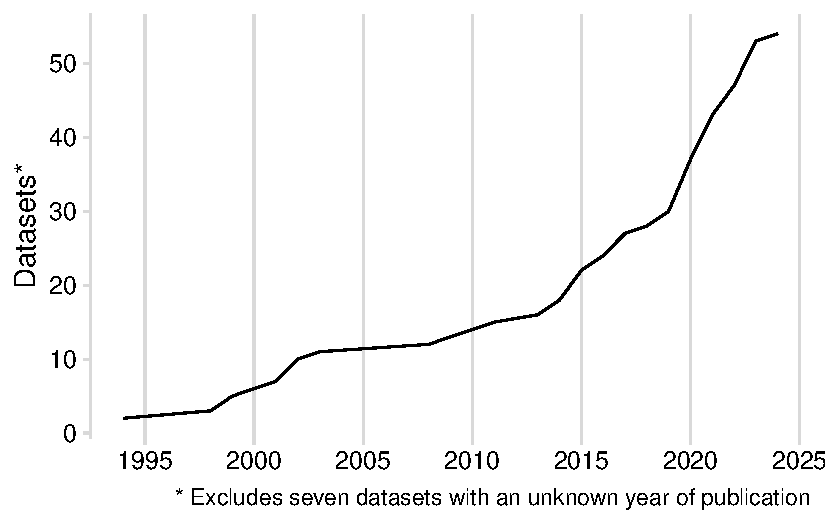
\includegraphics[keepaspectratio]{figures/fig-c14-datasets-time-1.pdf}}

}

\caption{\label{fig-c14-datasets-time}Cumulative number of radiocarbon
compilations published since 1995}

\end{figure}%

The number of available compilations has increased exponentially since
around 1995 (Figure~\ref{fig-c14-datasets-time}). The first generation
came around the turn of the century and consists mostly of online
databases with a web frontend. These include some databases operated by
radiocarbon labs, for example the Oxford Radiocarbon Lab (ORAU) and the
Belgian Royal Institute for Cultural Heritage (KIK-IRPA), and
essentially represent a continuation of their date lists in a digital
format. The majority, however, were compiled from the literature by
individual researchers interested in a particular region and/or period.
Notable early examples include ANDES 14C in 1994 (Central Andes,
Michczyński et al., 1995), CARD (Canada, Gajewski et al., 2011) and
RADON (Europe, Raetzel-Fabian, 1999) in 1999, and CANEW in 2001 (Near
East, Reingruber and Thissen, 2005). From 2010, coinciding with broader
shifts in scientific publishing (Tenopir et al., 2011), it became more
common to publish standalone `open data' products in the form of journal
supplements, archives in repositories and/or data papers; the
\emph{\href{https://openarchaeologydata.metajnl.com}{Journal of Open
Archaeology Data}}, launched in 2012, has been a prominent venue for
this latter category. Most recently there has been a trend towards
providing version-controlled plain text data via platforms such as
\href{https://github.com}{GitHub}, reflecting the broader adoption of
these tools amongst computational archaeologists over the last decade
(Batist and Roe, 2024). The shift from online databases towards more
static but more preservable open data products is welcome, given how
many databases from the first generation have subsequently ceased to be
accessible. Version-controlled repositories are particular well-suited
to data compilation projects because they allow for continued updates
whilst still providing snapshot `releases' that are citeable and can be
archived in long-term repositories.

\begin{figure}

\centering{

\pandocbounded{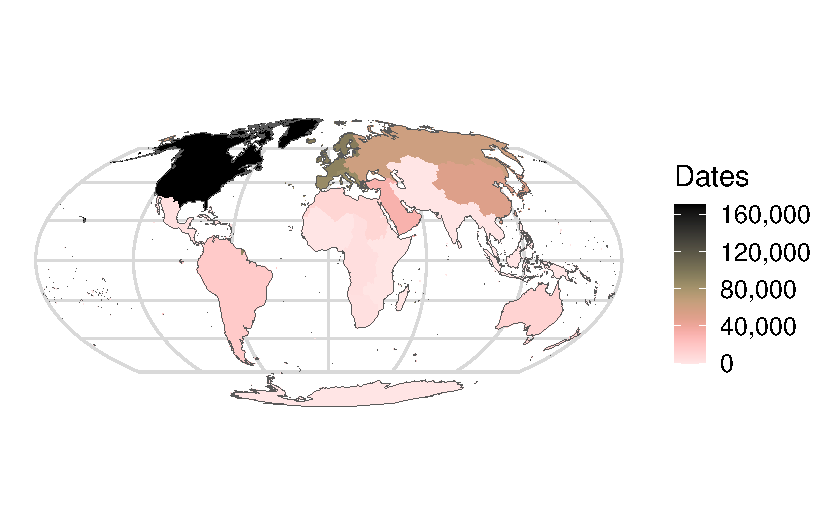
\includegraphics[keepaspectratio]{figures/fig-c14-datasets-map-1.pdf}}

}

\caption{\label{fig-c14-datasets-map}Geographic coverage of published
regional radiocarbon compilations according to our survey (see
Supplementary Material).}

\end{figure}%

Although this body of work has greatly improved the accessibility of
radiocarbon dates and supported significant methodological advances
(Crema et al., 2024; Crema, 2022), some limitations are apparent.

The geographic coverage of regional radiocarbon compilations is markedly
uneven (Figure~\ref{fig-c14-datasets-map}). Europe and, especially,
North America are over-represented (Alcántara and Pedroza, in press;
Chaput and Gajewski, 2016). South America, West Asia, and East Asia are
reasonably well-covered, but there practically no systematically
compiled dates from East or West Africa, Central or South Asia, or
Mainland Southeast Asia. This is probably explained in part by a lower
volume of archaeological research and access to radiocarbon dating in
these regions, but a lack of attention in compilation work must also be
a factor. For example, radiocarbon dating has been an established part
of Indian archaeology since at least 1961 (Kusumgar et al., 1963), but
we have not able to locate a single systematic compilation of dates from
South Asia.\footnote{We would be very happy to be corrected on this
  point.}

Datasets based on literature review also become out of date almost
immediately upon publication, due the the constant production of new
dates. Unfortunately this applies to many databases that are in theory
continuously updated, as it is common to see them become unmaintained
and or unexpectedly become unavailable. Of the 61 published datasets we
identified, 33 were intended to be continuously updated, but only 13
have received updates in the last two years. The average `lifespan' of a
dataset from its publication to its last update is around 4 years. Most
radiocarbon datasets we reviewed were compiled with a specific goal in
mind (e.g.~a particular analysis) and, even where there is the intention
to keep them updated afterwards, the exigencies of scientific production
combined with the labour-intensive nature of the process make that
difficult to achieve in practice.

Laboratory databases solve the problem of currency, but tend to have
more arbitary coverage, since the inclusion of data is determined by who
submits dates to that lab, not any form of principled curation. There
are also comparatively few of them -- most active labs no longer
directly publish dates that they produce (if they ever did).

Other outstanding problems with existing compilations include various
systematic biases in data collection (Clist et al., 2023) and a large
degree of overlap and duplication between individual databases. For
example, we identified 9 different resources covering Western Europe but
none covering South Asia. The quality and accessibility of published
compilations is also variable. 50 of the 61 resources we reviewed are
not `open' according to the Open Knowledge Foundation's definition of
data openness (``Open data and content can be freely used, modified, and
shared by anyone for any purpose,'' Open Knowledge Foundation, n.d.),
which both limits the access to and reuse potential of these datasets.
And even of these, many are not currently available in readily
machine-readable formats (e.g.~plain text or database files rather than
PDFs or hypertext).

The fragmentation of the radiocarbon record into regional datasets also
hinders analysis at larger scales. Although the core elements of a
radiocarbon date---laboratory identifier, radiocarbon age, measurement
error---are more or less standardised, there is no such consistency in
contextual information on the sample or site. Such contextual
information is important not just for the interpretation of dates, but
for filtering out unreliable dates based on sample information
(`chronometric hygiene' sensu Pettitt et al., 2003) and for correcting
for known systematic errors such as the marine reservoir effect (Alves
et al., 2018). Most published datasets incorporate all or part of
earlier compilations, meaning duplicate records are also very common,
but deduplicating them is not a trivial problem due to format variations
(see Section~\ref{sec-implementation-data}). These issues are by no
means impossible to overcome, but adds a significant amount of
data-cleaning effort to a process that would otherwise be very amenable
to standardisation.

\subsection{Global radiocarbon
compilations}\label{sec-global-compilations}

\begin{figure}

\centering{

\pandocbounded{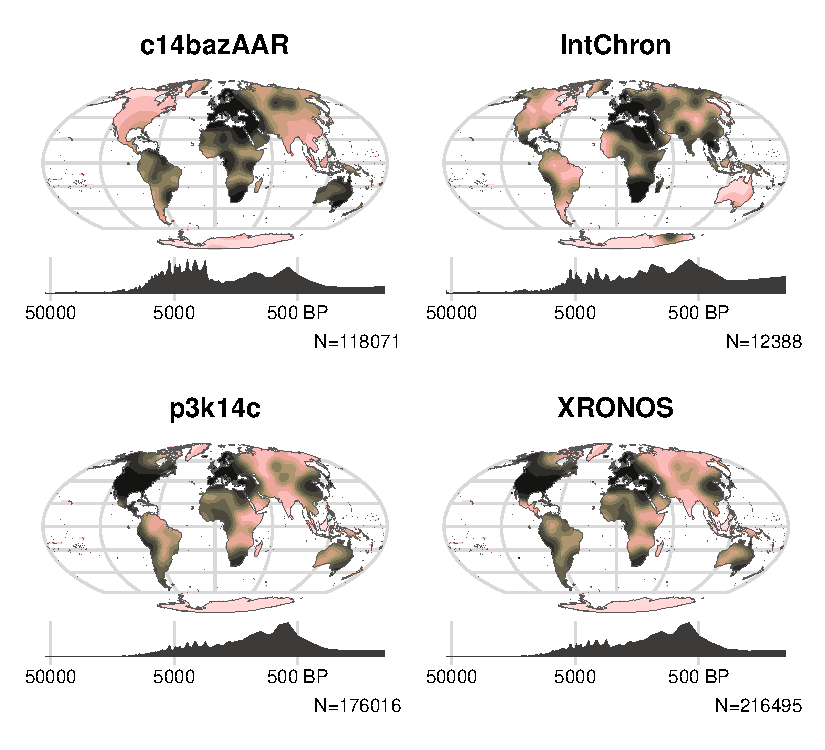
\includegraphics[keepaspectratio]{figures/fig-c14-global-1.pdf}}

}

\caption{\label{fig-c14-global}Geographic and temporal (sum calibration)
of georeferenced dates in XRONOS and other global radiocarbon
compilations}

\end{figure}%

The profusion of radiocarbon compilations over the last decade has
naturally prompted many to think globally. Three existing initiatives in
particular share similar aims to XRONOS (at least as far as radiocarbon
is concerned): c14bazAAR, IntChron, and p3k14c.

The first available synthetic radiocarbon database was c14bazAAR (Schmid
et al., 2019), an R package that provides an index of openly published
radiocarbon databases and a common interface for retrieving them and
performing basic data cleaning. Because c14bazAAR downloads data from
its original source repositories, rather than mirroring it, it only
includes resources that have been published in a fully open and
machine-accessible format. Despite this limitation, it has global
coverage and a large number of dates (Figure~\ref{fig-c14-global}), and
was therefore our starting point for data collection for XRONOS.

Another indexical approach is taken by the IntChron project (Bronk
Ramsey et al., 2019), which exposes data from multiple sources and
exposes them with a common JSON-based web interface. The IntChron
specification is open, meaning that radiocarbon labs or compilation
projects can implement it independently and thereby allow end users to
access their data through a common interface (though to our knowledge it
has so far only been adopted by databases associated with the Oxford
Radiocarbon Lab). The JSON format also lends itself to the
implementation of wrapper libraries, for example the rIntChron package
gives direct access to IntChron-indexed databases in R (Roe, 2024).

p3k14c (Bird et al., 2022) instead compiles multiple source databases
into a single flat file dataset, with a similar level of coverage to
c14bazAAR. The major advantage of this approach is that the data is made
internally consistent and has been manually cleaned to an extent, which
makes it particularly well-suited to global analyses. The downside is
that without the continuous link to the source databases present in the
c14bazAAR and IntChron, it can only be kept up to date manually with
periodic re-releases. An accompanying package (Bird et al., 2024)
provides direct access to the p3k14c dataset in R.

As of December 2024, c14bazAAR had 118,071 radiocarbon dates with unique
laboratory identifiers (excluding those sourced from p3k14c and XRONOS),
IntChron had 12,388 (excluding those from non-archaeological contexts),
and p3k14c had 176,016. The geographic distribution of dates from each
is similar (Figure~\ref{fig-c14-global}), reflecting the large degree in
overlap between the sources of each compilation. IntChron, which in
practice is currently only used to publish dates associated with the
Oxford Radiocarbon Lab, has dates from more diverse contexts, but is an
order of magnitude smaller.

\subsection{Beyond radiocarbon}\label{beyond-radiocarbon}

Radiocarbon has been by far the most active area of open data
compilation, but archaeological chronology incorporates a much more
diverse range of sources of information (Harding, 1999). In periods
beyond the practical limit of radiocarbon dating (c.~55,000 BP), other
types of radiometric (K--Ar, U--Pb, etc.), chemical or luminescence
dating offer an alternative (Aitken, 1999). Conversely, in historic
periods, radiocarbon is often relatively underused compared to
conventional typological dating (based on artefact characteristics),
which in these periods can offer comparable or better temporal
resolution, or direct dating based on epigraphy (Heřmánková et al.,
2021), numismatics (Kemmers and Myrberg, 2011) or historical sources. In
places where it is widely available, dendrochronology (Baillie, 2014)
also produces significantly better resolved chronologies and therefore
tends to be the main source of chronometric data. Other more
application-specific chronological methods include shoreline dating
(Brøgger, 1905; Roalkvam, 2023), lichenometry (Benedict, 2009) and rock
weathering dating (Bednarik, 2020; Whitley, 2012).

Compared to radiocarbon, there are few examples of systematic, open
compilations of any of these other types of data. This is most striking
when it comes to other radiometric/scientific dating methods, as the
data structures and publication modes are very similar to radiocarbon.
The `Radiocarbon Palaeolithic Europe Database' (Vermeersch, 2020),
despite the name, includes a significant number of thermo- and optically
stimulated luminescence, electon spin resonance, uranium--thorium and
amino acid dates. Similarly, the AustArch database (Williams et al.,
2014) includes luminescence dates alongside radiocarbon, but is limited
to Australia and was last updated in 2013. Apart from these and a few
other exceptions where other scientific dates are collected alongside
radiocarbon, we are not aware of any open compilations of them.

\subsubsection{Dendrochronology}\label{dendrochronology}

With regard to tree-ring data, some databases provide valuable resources
for dendrochronological studies in general but are not primarily
intended for archaeological contexts. For instance, Dendro4Art
specializes in dendrochronological data related to wooden art objects,
such as sculptures and panel paintings. While this focus serves art
historians and conservationists well, its utility for studying
prehistoric datasets is minimal. Similarly, the Dendrochronological
Picture Database, maintained by the Swiss Federal Institute for Snow and
Avalanche Research (SLF), offers a visual archive of approximately 1,400
images documenting dendrochronological phenomena. Although valuable as
an educational resource, it does not provide raw data necessary for
chronological or archaeological analyses. Additionally, the OLDLIST and
Eastern OLDLIST databases focus on documenting the maximum ages of trees
worldwide. Their emphasis on biological longevity, while significant for
ecological research, limits their applicability to archaeological or
prehistoric investigations.

Among databases that do provide dendrochronological data, the degree to
which they support prehistoric research varies substantially. The NOAA
International Tree-Ring Data Bank (ITRDB) serves as a global repository
of tree-ring measurements. However, its focus remains predominantly on
North America, with only 34 datasets representing European prehistoric
contexts. This restricts its relevance for studying the European past.
Similarly, the ADS database, maintained by the UK-based Vernacular
Architecture Group, compiles dendrochronological data from the UK but is
limited to medieval and later periods, making it unsuitable for
prehistoric studies.

DendroDB, hosted by the Swiss Federal Institute for Forest, Snow and
Landscape Research (WSL), emphasizes ecological and climate studies over
archaeological wood material. While it claims a broad scope, the
database remains non-functional, rendering it ineffective for research
needs. The CFS-TRenD database, managed by the Canadian Forest Service,
compiles over 4,600 datasets from Canadian forests, primarily focusing
on boreal ecosystems. Despite its extensive coverage for North America,
its geographical specificity and lack of open access restrict its
utility for European prehistoric contexts. Similarly, the QUB
Dendrochronology Database, managed by Queen's University Belfast, offers
valuable datasets for Ireland and the UK but lacks significant
representation of prehistoric material, limiting its application in
broader archaeological investigations. The Building Archaeology Research
Database (BARD) contains over 24,000 records, including
dendrochronological data from more than 2,700 buildings. However, its
focus on medieval and post-medieval timber-frame construction further
narrows its utility for studies involving prehistoric wood samples.

The Digital Collaboratory for Cultural Dendrochronology (DCCD) presents
itself as a potentially valuable international platform for
dendrochronology, particularly through its integration with
archaeological data services such as ARIADNE. However, it remains
heavily biased toward datasets from the Netherlands, which account for
more than two-thirds of its entries, while only 0.08\% of its
\emph{Quercus} data pertain to Switzerland and just 2.5\% represent
prehistoric datasets. Notably, these estimates date back to 2021, and an
updated assessment is currently unattainable following the platform's
migration to DataverseNL, which now charges an annual fee of nearly
€6,000 for access. Furthermore, database activity has declined
significantly, from 3,846 new project records between 2010 and 2014 to
only 83 by the end of 2019. Although 519 additional records have been
reported since 2021, it remains unclear whether this figure includes
revisions to pre-existing entries, potentially inflating the count. The
database's narrow focus and restrictive access model significantly limit
its broader utility for prehistoric research.

Finally, the Strategic Environmental Archaeology Database (SEAD), hosted
by Umeå University, integrates multiple environmental proxies, including
dendrochronological data. However, the dendrochronological component is
largely confined to Swedish data, with limited relevance to prehistoric
contexts. While SEAD aims for broader applications, its dendro component
has limited utility for studies outside Sweden.

The utility of dendrochronological databases for prehistoric research
varies widely. Global resources such as NOAA's ITRDB and DCCD offer
substantial datasets but face significant limitations in practical
geographical and temporal scope. Similarly, platforms like DendroDB and
BARD primarily cater to historical studies, leaving critical gaps in
prehistoric coverage. Specialized resources like OLDLIST, Dendro4Art,
and the Dendrochronological Picture Database provide valuable
contributions but lack the direct relevance necessary for archaeological
tree-ring analysis. Consequently, researchers focused on prehistoric
dendrochronology must navigate a fragmented landscape of databases, each
offering distinct strengths and limitations. Addressing these gaps
remains crucial for advancing the field.

\subsubsection{Typological dating}\label{typological-dating}

Typological dates---i.e.~relative, expertise- or seriation-based dating
based on artefact characteristics---are ubiquitous in archaeological
studies but rarely treated as a form of chronometric data in their own
right. For example, the majority of the radiocarbon datasets we reviewed
(Section~\ref{sec-c14-compilation}) included some form of typological
chronological information in the form of a `period' or `culture' column.
This is also typically present in many other forms of systematic
compilation work in archaeology, for example site gazetteers. Aggregated
typological information from such sources are often used in aoristic
analysis and related methods (Crema, 2024; Mischka, 2004). What is
lacking in this presentation of typological dating is metadata on how
the determination was made and how exactly it is to be understood. Like
any archaeological date, a typological date is derived from a physical
sample -- the object or set of object from which a chronological
estimate was derived. Typological dates on one class of object may well
clash with other classes of object, or for that matter with scientific
dates -- does one trust the date on pottery, the date on architecture,
or the radiocarbon date? Without additional metadata on e.g.~who made
the typological determination or what the radiocarbon date was obtained
on, such inconsistencies are difficult to resolve Similarly the absolute
date range corresponding to a typological determination (e.g.~``Late
Neolithic'') can be interpreted in multiple ways depending on the region
and intentions of the expert making the determination. PeriodO
(Rabinowitz et al., 2016) is a linked open data infrastructure that
includes a shared vocabulary of typological periods and corresponding
calendar age estimates, and an important step towards addressing the
latter problem. However, it remains to be systematically linked to
compilations of typological dates (though there are some efforts in this
direction e.g. Hannah et al., 2022).

\begin{center}\rule{0.5\linewidth}{0.5pt}\end{center}

What is missing to date is a general-purpose infrastructure for
combining all of these types of chronometric information on a global
scale. This is the gap that XRONOS aims to fill, starting with three
methods: radiocarbon, dendrochronology, and typological dating. These
were chosen because they are widely used and relatively advanced in
terms of open data, but an important aim of the project is to develop a
generalisable data model that can easily scale to any and all types of
archaeological chronology (see Section~\ref{sec-data-model}).

\section{Concept}\label{concept}

XRONOS inherits its basic structure from RADON (Hinz et al., 2012;
Kneisel et al., 2014; Raetzel-Fabian, 1999; Rinne et al., 2024), with a
database-backed web application and a data model that separates
radiocarbon dates, contextual information, and sites. Our overall aims
in developing XRONOS is to bring this model, which RADON has operated on
for more than twenty years, up to date, to generalise it to other types
of chronometric information, and to transform it from an online database
to a data infrastructure that supports the continuous ingestion,
curation, and open dissemination of archaeological chronologies from
diverse sources.

\subsection{Design goals}\label{design-goals}

XRONOS is our answer to Kintigh's call (Kintigh, 2006) for digital
infrastructures that don't just provide access to chronological data but
enables researchers to ``archive, access, integrate, and mine disparate
data sets''. It complements several similar open data infrastructures
within and outwith archaeology, such as the Global Biodiverisity
Information Facility (GBIF, Canhos et al., 2004), the Strategic
Environmental Archaeology Database (SEAD, Buckland, 2014), IMPACT for
mummified human remains (Nelson and Wade, 2015), Neotoma for
palaeoecological data (Williams et al., 2018), IsoArcH for stable
isotope data (Plomp et al., 2022), the International Soil Radiocarbon
Database (ISRaD, Lawrence et al., 2020), and the `Big Interdisciplinary
Archaeological Database' (BIAD), an ambitious new initiative to combine
many of these individual domains, including chronology (Reiter et al.,
2024). To improve upon existing global syntheses of radiocarbon dates
(see Section~\ref{sec-global-compilations}), we aimed to develop a
living infrastructure that both continually collected data from diverse
sources and presented a seamless single database to the user.

Our principal goals for the software were therefore to:

\begin{enumerate}
\def\labelenumi{\arabic{enumi}.}
\tightlist
\item
  Combine all available sources of radiocarbon and other chronometric
  data in single database
\item
  Develop robust tools for the continuous ingestion, collation and
  curation of this data
\item
  Disseminate the collated and curated data as linked open data within a
  FAIR framework
\end{enumerate}

Meeting these goals required the development of a) a conceptual data
model, including links to other open data resources, that is flexible
enough for all forms of chronometric data; and b) a software
implementation that supports the main functions of ingesting, curating,
and disseminating this data. The individual components of this work are
described in more depth below but, briefly, consist of a relational data
model implemented in a PostgreSQL database; a Ruby application providing
server-based tools for ingestion, curation and dissemination of data;
and multiple graphical and programmatic interfaces to the resulting
dataset.

\subsection{Data model}\label{sec-data-model}

\begin{figure}

\centering{

\pandocbounded{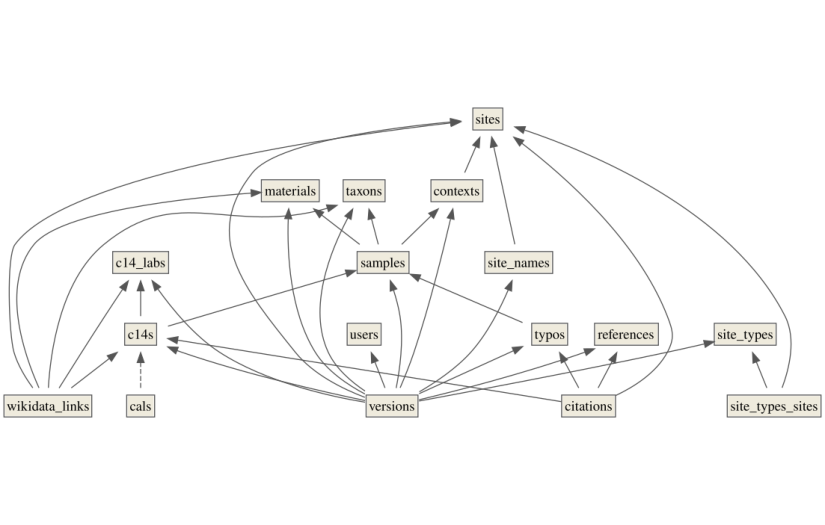
\includegraphics[keepaspectratio]{figures/fig-data-model-1.pdf}}

}

\caption{\label{fig-data-model}Simplified entity relationship diagram
showing the XRONOS data model}

\end{figure}%

At the base of the XRONOS data model (Figure~\ref{fig-data-model}) are
sets of spatiotemporal coordinates or, as we call them, \emph{chrons}.
In an archaeological context, we conceptualise a chron as an assertion
linking human activity with a particular point in space and time. Our
data model currently encompasses three types of chron: radiocarbon
dates, typological dates (e.g.~`Early Neolithic') and
dendrochronological dates. However we anticipate that the concept will
accommodate other types of absolute and relative dating techniques, as
the scope of the database expands.

Chrons are conceptually useful because they emphasise that different
types of archaeological `dates', drawn from different sources, have
essentially the same information content: the location of an event in
space and time. We thereby avoid privileging certain sources of
chronological data over (as might be the case if, for example, we
treated `period' as a fixed attribute of a site) and can accommodate
contradictory (e.g.~differences of opinion on typological
classification). This is important given that XRONOS aspires to be an
authoratative `backbone' with a global scope, so we cannot realistically
impose a single chronological scheme or resolve conflicting information
provided by specialists. They are useful practically because they expose
a common interface for attributes that all types of chronological
information share, such as a \emph{terminus post quem} (TPQ),
\emph{terminus ante quem} (TAQ), and midpoint estimate. This allows
applications that use XRONOS' data model (including XRONOS itself) to
collate chronological data from multiple sources, without necessarily
having to be aware of the pecularities of each type of dating.

In order to unify chronological information in the form of a chron, we
need a common chronological `coordinate system'. The natural choice is a
\emph{calendar probability distribution}, which expresses the
probability that an event occurred as a function of time on a calendric
scale. Most archaeologists are familiar with working with this kind of
representation in the form of calibrated radiocarbon dates, but it can
be extended and generalised to essentially any kind of chronological
information. For example, in aoristic analysis (Mischka, 2004), a
periodic time estimate (e.g.~the event occurred in the Neolithic) is
conceptualised as a uniform probability distribution over the timespan
between the known start and end dates of that period. A similar model is
used in OxCal (Bronk Ramsey, 2009, a direct inspiration for our
approach) to integrate prior chronological information from diverse
sources. In practical terms, this model means that the canonical
representation the time component of any chron in XRONOS, regardless of
source, is a probability distribution over the set of calendar years
(arbitrarily measured in years Before Present) in which it could have
plausibly occurred. Further statistics, e.g.~a midpoint estimate or
TPQ/TAQ range, can be derived from this distribution using well-known
methods. In this way, we can support many different types of date and
much of the implementation of XRONOS can be agnostic to the source of
chronological information.

Chrons are located in space through association to a \emph{sample} --
the physical object from which a chronological determination was made.
The location of samples is represented with geographical coordinates and
an associated coordinate reference system (CRS), though since in
practice the precise location of single samples is rarely available,
this property is usually inherited from the site. We also record
relevant metadata on the nature of the sample. For radiocarbon dates,
for example, we follow established conventions (Millard, 2014) in
recording the type (e.g.~charcoal, charred seed) and, where applicable,
taxonomic designation (e.g.~\emph{Quercus}, \emph{Triticum dicoccum}) of
the organic material used for dating. For typological dates, an ideal
scenario would be for the sample to represent the particular object from
which an inference was made (e.g.~`Natufian' might be inferred from
`lunate-type microlith'). In practice, the best we can glean from most
published datasets is the type of material used (e.g.~`pottery',
`lithics'). The same sample can be associated with multiple chrons,
including different types of chron. This is useful, for example, for
representing replicate radiocarbon dates on the same sample, or
radiocarbon dates and dendrochronological made on the same section of
wood for wiggle-matching.

Further contextual information is associated with \emph{contexts} and
\emph{sites}. The site is the primary geographic container for
chronological information. As already mentioned, we typically record the
spatial location of chrons using this entity, though it is possible to
modify this by providing specific coordinates at the sample level. Sites
also have attributes describing their conventional name or names in
different languages and are associated with a flexible `site type'
typology that combines information on their form and function.

A context represents the specific find-context of a sample, e.g.~an
architectural feature, stratigraphic unit, or phase. Since the units and
conventions for recording such information vary greatly between
different regions and archaeological traditions---and XRONOS is designed
with global data in mind---we leave the question of what a context
precisely represents open, and only record an unstandardised, free text
label for it. Crucially, however, contexts can have a self-referential
association to other contexts belonging to the same site. This allows it
to encode arbitrary relational structures between contexts, whether they
be hierarchical (e.g.~phases and sub-phases) or graphical
(e.g.~stratigraphic). In this way, it can serve as a foundation for
chronological modelling.

The series of relations
\texttt{{[}chron{]}\ \textgreater{}\ sample\ \textgreater{}\ context\ \textgreater{}\ site}
links the chronological and contextual sides of the XRONOS data model.
Each step is a many-to-one association, meaning for example that it is
possible to attach multiple chrons to the same sample (e.g.~replicated
radiocarbon dates on the same material), multiple \emph{types} of chrons
to the same sample (e.g.~radiocarbon dates on tree-rings for
wiggle-matching). Since this kind of information is rarely
systematically recorded in our source databases, there are currently few
actual records that make use of this feature of the data model. However,
we hope it will provide a foundation for more nuanced chronological
modelling in the future.

Metadata is incorporated into XRONOS' data model at the level of the
individual records (e.g.~all records store their data of creation and
last modification) and through two additional types of record:
bibliographic \emph{references} and \emph{versions}. Bibliographic
references store information on the source of a record in BibTeX format
and can be linked through many-to-many associations to sites or chrons.
Versions are a special type of record that are associated with all other
records (including bibliographic references) and store the previous
versions of those records as a series of changesets. In this way all
changes to data are recorded and can be reconstructed (or reversed)
precisely. This `paper trail' also stores contextual metadata, e.g.~who
made the change and why. It also means that records that are deleted can
be reviewed or restored from their stored version history, which is
never discarded. Together these two systems provide a transparent record
where the data in XRONOS comes from and how it has been altered, which
we view as essential in a scientific data infrastructure.

\subsection{Linked data}\label{linked-data}

The XRONOS data model presents several opportunities to link to other
resources as linked open data (LOD). We use controlled vocabularies such
as the GBIF Backbone Taxonomy (GBIF Secretariat, 2023, for taxonomic
descriptions of samples) to both standardise fields and to link the two
resources based on this shared concept. There are concordances between
XRONOS entities and several other specialised data infrastructures in
archaeology, such as PeriodO (Rabinowitz et al., 2016, mapping to
typological chrons) and gazetters like Pleiades (Bagnall et al., 2006)
or Vici (Voorburg, 2012, mapping to site names). Moving beyond
archaeology, Wikidata (\url{https://wikidata.org}) already includes many
of the concepts represented in the XRONOS model (e.g.~an `archaeological
site', \url{https://www.wikidata.org/wiki/Q839954}). Linking to Wikidata
is especially useful because it dissimenates---and thereby
preserves---the data compiled in XRONOS beyond the specialist/academic
community. It also allows us to enrich the database with contextual
information that otherwise be beyond our scope and resources, for
example embedding multilingual descriptions of sites from Wikipedia
articles on site records where the site has been linked to a Wikidata
item.

Conversely, we encourage others to use XRONOS as a linked open data
resource by providing stable URLs and a machine-readable interface for
every record. Such usages could look like, for example, using a XRONOS
URL as a canonical representation of a single radiocarbon date
(e.g.~\url{https://xronos.ch/c14s/SMU-257} -\textgreater{}
\url{https://xronos.ch/c14s/23410}). We also plan to implement
additional view formats to facilitate this, such as IntChron-format
JSON, to allow it to be indexed through the IntChron service, or RDF,
which is widely used by many linked open data resources in the digital
humanities.

\section{Implementation}\label{implementation}

Following a short pilot project in 2019, the first phase of development
of XRONOS was completed in 2021--2024. The web interface
(\url{https://xronos.ch}) has been publicly accessible since July 2021.
Though we envisage XRONOS as a continuously-developing open source
project and `living database', the following offers a snapshot of
progress at the end of our first grant-funded implementation phase. We
do not aim to be comprehensive, but rather to describe some key elements
of XRONOS' current implementation that illustrate how our concept has
been realised in practice.

\subsection{Software architecture}\label{software-architecture}

The XRONOS data model is implemented as a relational database using the
free and open source database management system PostgreSQL. However,
apart from backups and other routine maintenance procedures, all
interaction with the database is via a web application, which thus forms
the core of XRONOS' architecture. The XRONOS web application is written
in Ruby and uses CRUD (Create, Read, Update, Delete) and MVC (Model,
View, Controller) patterns as implemented in the Ruby on Rails
framework.

The XRONOS web application exposes two distinct user interfaces: a
graphical user interface accessed through a web browser; and an
application programming interface (API). Both interfaces follow a REST
(Representational State Transfer) pattern (Verborgh et al., 2015), where
each resource (e.g.~a single radiocarbon date, a single bibliographic
reference, or a single user) is statelessly mapped to a single address.
Users can then interact with resources at these addresses using a
preditable and uniform interface based on HTTP verbs. For example, the
radiocarbon date RTD-8904 is represented by the address
\url{https://xronos.ch/c14s/156205}. Users can view information on this
resource by sending a GET request to that address, regardless of which
interface they are using, and authorised users can modify it using POST,
PATCH, or DELETE requests. The bibliographic reference associated with
this date (Richter et al., 2017) is similarly represented at the address
\url{https://xronos.ch/references/17778}, and can be accessed at that
address using the same interface as the radiocarbon date. These uniform
REST interfaces are another example of a boring architectural choice
that make it easier for us to enrich the scientific contents of XRONOS,
by adding new types of modular resource that represent new scientific
entities.

This basic REST pattern is augmented by seven `actions' (following the
standard pattern in Rails application) that express different ways of
interacting with a resource: index, show, destroy, new, create, edit,
and update. The `show' action represents interaction with a single
resource, as described above. The `index' action, which lists resources
of a given type (e.g.~\url{https://xronos.ch/c14s} for radiocarbon
dates), is worth special mention because it is through this that the
filtering logic at the core of XRONOS' two interfaces is implemented. By
passing a query as HTTP GET parameters to the index action of a
resource, the list returned the user is modified to only include records
that match that query. For example,
\url{https://xronos.ch/sites?site\%5Bcountry_code\%5D=CH} (the part of
the URL after the \texttt{?} character encodes the SQL WHERE clause
\texttt{country\ =\ \textquotesingle{}CH\textquotesingle{}} as a GET
parameter) lists sites in Switzerland. More complex queries can be
executed using nested parameters. For example,
\url{https://xronos.ch/c14s?sample\%5Bmaterial\%5D\%5Bname\%5D=charcoal}
(encoding that the \texttt{c14} table should be joined to the
\texttt{material} table via \texttt{sample}, followed by the WHERE
clause
\texttt{material.name\ =\ \textquotesingle{}charcoal\textquotesingle{}})
lists radiocarbon dates obtained from charcoal samples. Index actions
can also respond with the result in a tabular data format
(i.e.~\texttt{.csv}).

\subsection{Data ingestion and curation}\label{sec-implementation-data}

The chronological data in XRONOS comes from a variety of sources,
including published structured datasets in repositories and journal
supplements, other online databases, literature review, and direct input
from collaborators. Our aim is not just to `mirror' these sources as
they are, but integrate them into a single curated and continuously
updated database. For the purposes of ingestion, we classify data
resources into three categories: static resources, such as supplementary
data in published papers, which are imported once; versioned resources,
updated on a periodic basis, which we import after each new version; and
live resources, which are continuously updated and therefore
continuously imported. Records of each type are imported into XRONOS in
as close to their original state as possible, i.e.~without any
corrections or standardisation applied. This ensures that any subsequent
changes (even immediate, automatic ones) are entered into the record's
version history, so that the source of any deviations or potential
errors can always be reconstructed. The version history also records the
direct source of the data for attribution purposes. In addition, a
bibliographic reference to the original resource is attached to ensure
that the source is clearly attributed even if the record is merged with
another one.

\begin{table}

\caption{\label{tbl-issues}Automatically-recognised data quality issues
currently implemented in XRONOS}

\centering{

\fontsize{9.8pt}{11.7pt}\selectfont
\begin{tabular*}{\linewidth}{@{\extracolsep{\fill}}>{\raggedright\arraybackslash}p{\dimexpr 0.30\linewidth -2\tabcolsep-1.5\arrayrulewidth}>{\raggedleft\arraybackslash}p{\dimexpr 0.20\linewidth -2\tabcolsep-1.5\arrayrulewidth}>{\raggedright\arraybackslash}p{\dimexpr 0.50\linewidth -2\tabcolsep-1.5\arrayrulewidth}}
\toprule
Issue & N & Description \\ 
\midrule\addlinespace[2.5pt]
\multicolumn{3}{l}{Sites} \\[2.5pt] 
\midrule\addlinespace[2.5pt]
MISSING\_COORDINATES & 4452 & Missing geographic coordinates \\ 
INVALID\_COORDINATES & 0 & Geographic coordinates fall outside the earth's ellipsoid \\ 
MISSING\_COUNTRY\_CODE & 1221 & Missing data on what country the site is in \\ 
\midrule\addlinespace[2.5pt]
\multicolumn{3}{l}{Samples} \\[2.5pt] 
\midrule\addlinespace[2.5pt]
MISSING\_MATERIAL & 138177 & Missing data on the sample material \\ 
MISSING\_TAXON & 138182 & Missing data on the sample taxon \\ 
MISSING\_CRS & 0 & Sample has coordinates but the coordinate reference system is not given \\ 
\midrule\addlinespace[2.5pt]
\multicolumn{3}{l}{Taxons} \\[2.5pt] 
\midrule\addlinespace[2.5pt]
UNKNOWN\_TAXON & 9260 & Sample taxon has not been matched to the GBIF Backbone Taxonomy \\ 
LONG\_TAXON & 509 & Description of the sample taxon is implausibly long \\ 
\midrule\addlinespace[2.5pt]
\multicolumn{3}{l}{Radiocarbon dates} \\[2.5pt] 
\midrule\addlinespace[2.5pt]
MISSING\_C14\_AGE & 447 & Missing radiocarbon age \\ 
VERY\_OLD\_C14 & 76 & Radiocarbon age older than the effective range of the method (50 ka) \\ 
MISSING\_C14\_ERROR & 585 & Missing measurement error \\ 
MISSING\_D14C & 238875 & Missing δ13C measurement \\ 
MISSING\_D14C\_ERROR & 238875 & Missing δ13C measurement error \\ 
MISSING\_C14\_METHOD & 242233 & Missing data on radiocarbon dating method (conventional, AMS, etc.) \\ 
MISSING\_C14\_LAB\_ID & 1233 & Missing laboratory identifier \\ 
INVALID\_LAB\_ID & 16053 & Laboratory identifier does not match the standard format (e.g. 'Abc-1234') \\ 
MISSING\_C14\_LAB & 350190 & Missing data on the radiocarbon laboratory \\ 
\midrule\addlinespace[2.5pt]
\multicolumn{3}{l}{Bibliographic references} \\[2.5pt] 
\midrule\addlinespace[2.5pt]
MIXED\_REFERENCE & 21933 & Bibliographic reference appears to combine multiple publications \\ 
MISSING\_BIBTEX & 42109 & Bibliographic reference without structured data in BibTeX format \\ 
\bottomrule
\end{tabular*}

}

\end{table}%

Once ingested, we apply a number of automated and semi-automated quality
control processes to integrate new data into the existing database.
Controlled vocabularies are used in a number of places in the data model
(Figure~\ref{fig-data-model}), and we use thesauri to automatically
standardise these fields as much as possible. For example, as mentioned
above, the taxonomic description of samples is controlled using GBIF's
backbone taxonomy (GBIF Secretariat, 2023), and we also use a thesaurus
service provided by GBIF to automatically change variant or obsolete
taxonomic names to the canonical version. If the system is not able to
standardise a field using the available thesaurus, it is flagged for
manual correction. A wide variety of other potential data quality issues
(e.g.~missing data on what country a site is in) are also flagged for
human review by this system Table~\ref{tbl-issues}, which can often be
semi-automated (e.g.~suggesting close matches in the thesaurus or the
country indicated by the record's coordinates).

A final critical component of XRONOS' data curation system is duplicate
handling. We import data from many overlapping resources (many of which
incorporate each other either in whole or in part), so duplicate records
are common (as recently discussed by Reiter et al., 2024). The end
result of standardising and correcting a record is also often to create
a duplicate: e.g.~the same sample imported from one source as `oak' but
another as `\emph{Quercus} sp.' will become a duplicate pair as
`\emph{Quercus}', and thus be recognised as a single sample. Such exact
duplicates can be merged automatically, with the oldest record becoming
the authoratitive version, but detecting fuzzier duplicated information
(e.g.~differences in the spelling of site names) has proved a more
difficult problem. As of writing there are therefore still many
duplicate records in XRONOS that need to be manually resolved, but we
hope to automate much more of this work in the future.

\subsection{User interfaces}\label{user-interfaces}

\begin{figure}

\begin{minipage}{0.50\linewidth}

\centering{

\pandocbounded{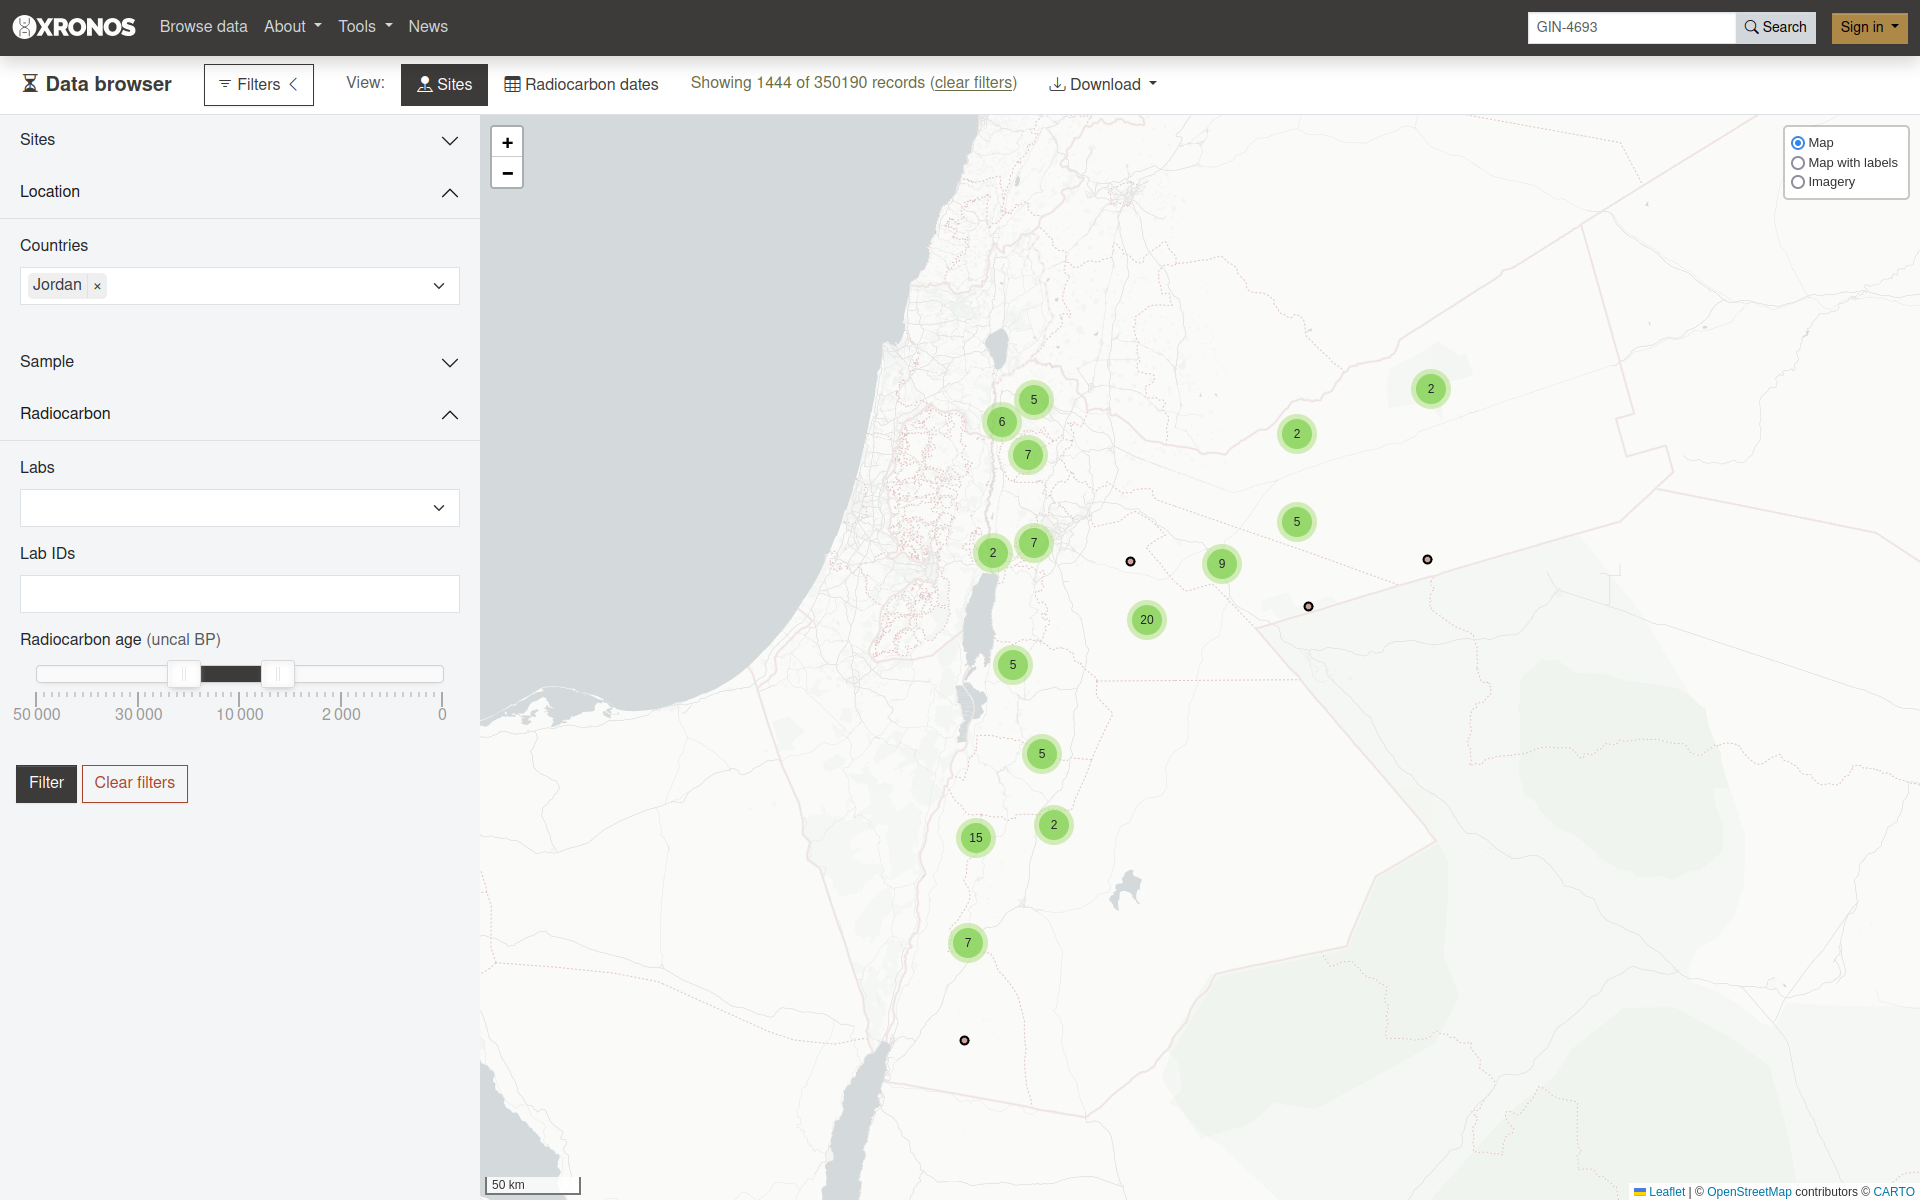
\includegraphics[keepaspectratio]{figures/xronos-ui-data-browser.png}}

}

\subcaption{\label{fig-ui-data-browser}Data browser}

\end{minipage}%
%
\begin{minipage}{0.50\linewidth}

\centering{

\pandocbounded{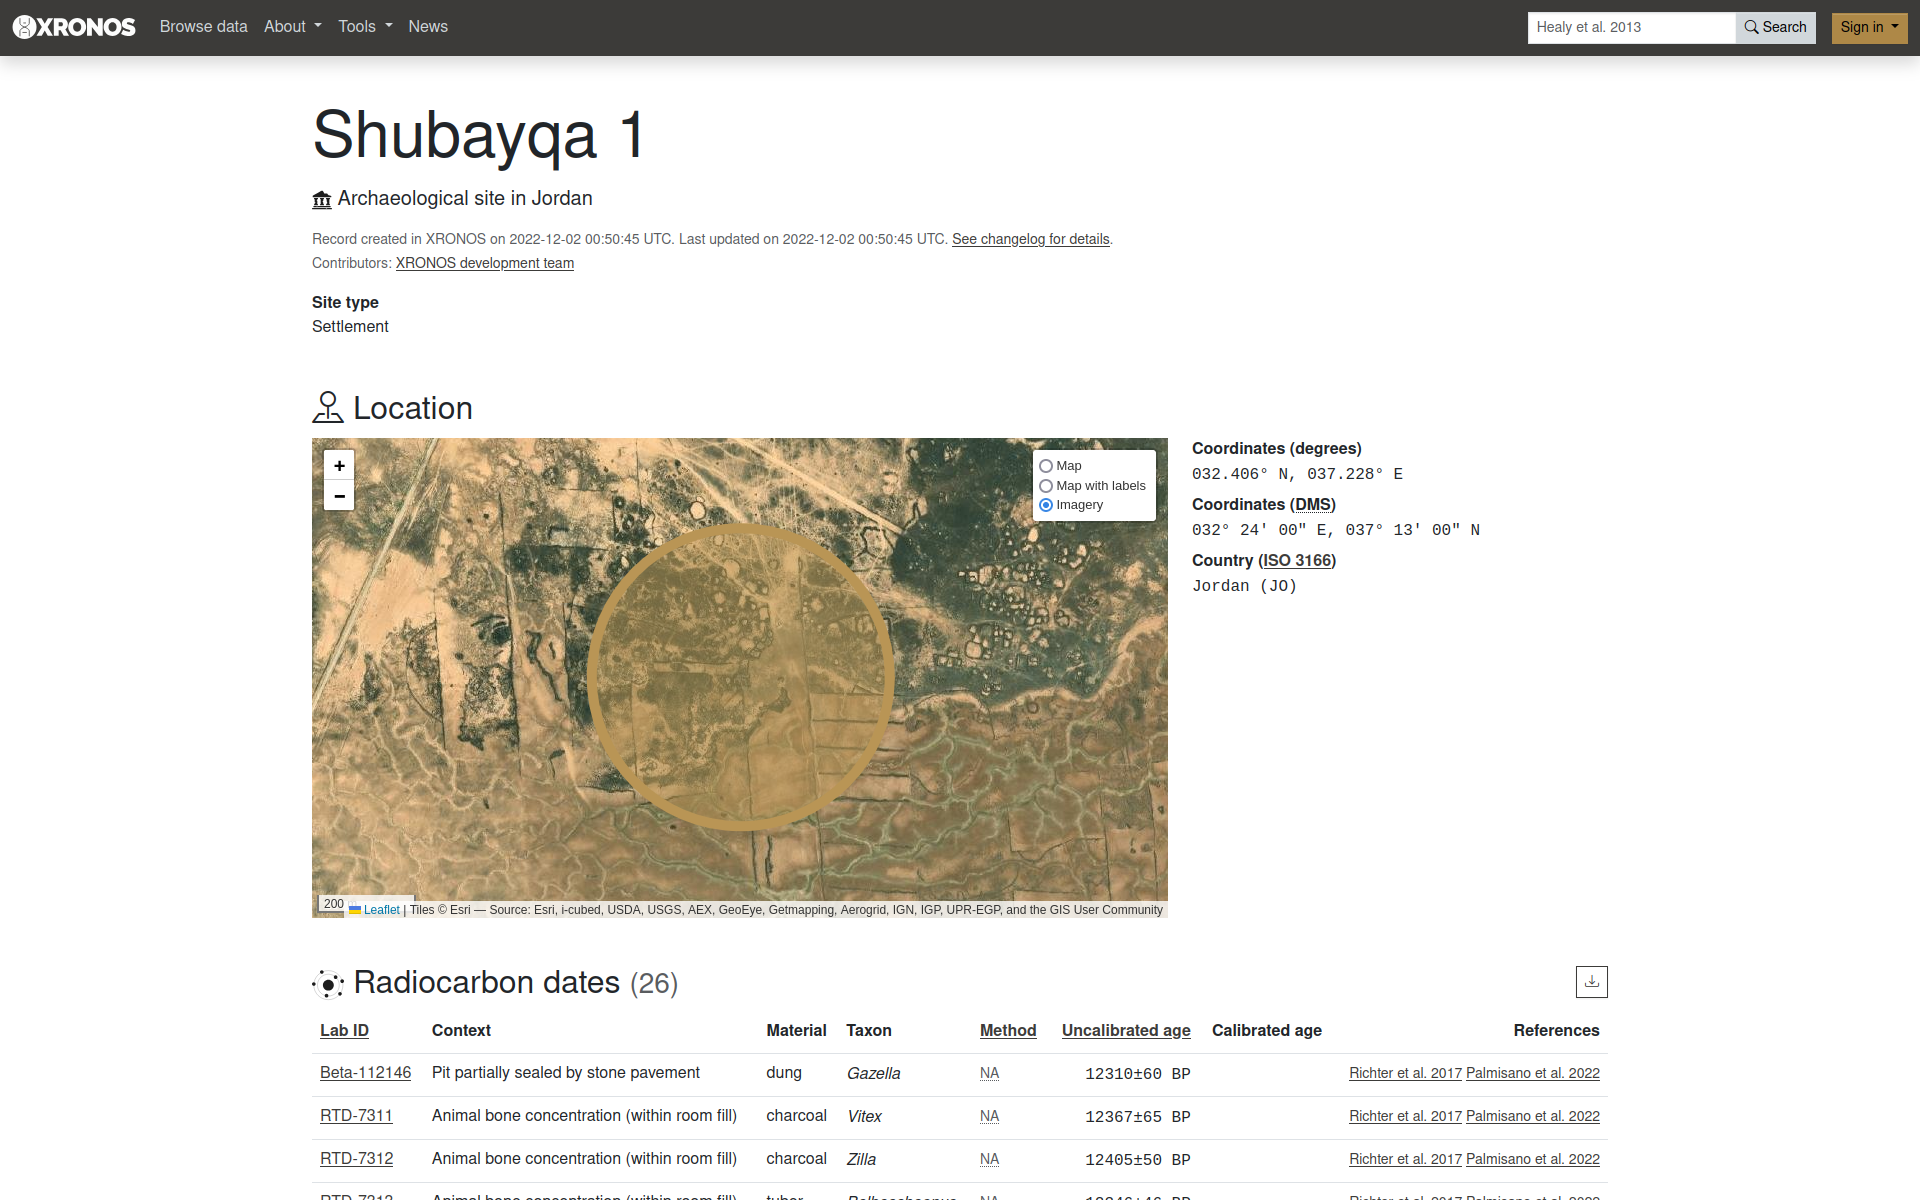
\includegraphics[keepaspectratio]{figures/xronos-ui-show.png}}

}

\subcaption{\label{fig-ui-show}Site record}

\end{minipage}%
\newline
\begin{minipage}{0.50\linewidth}

\centering{

\pandocbounded{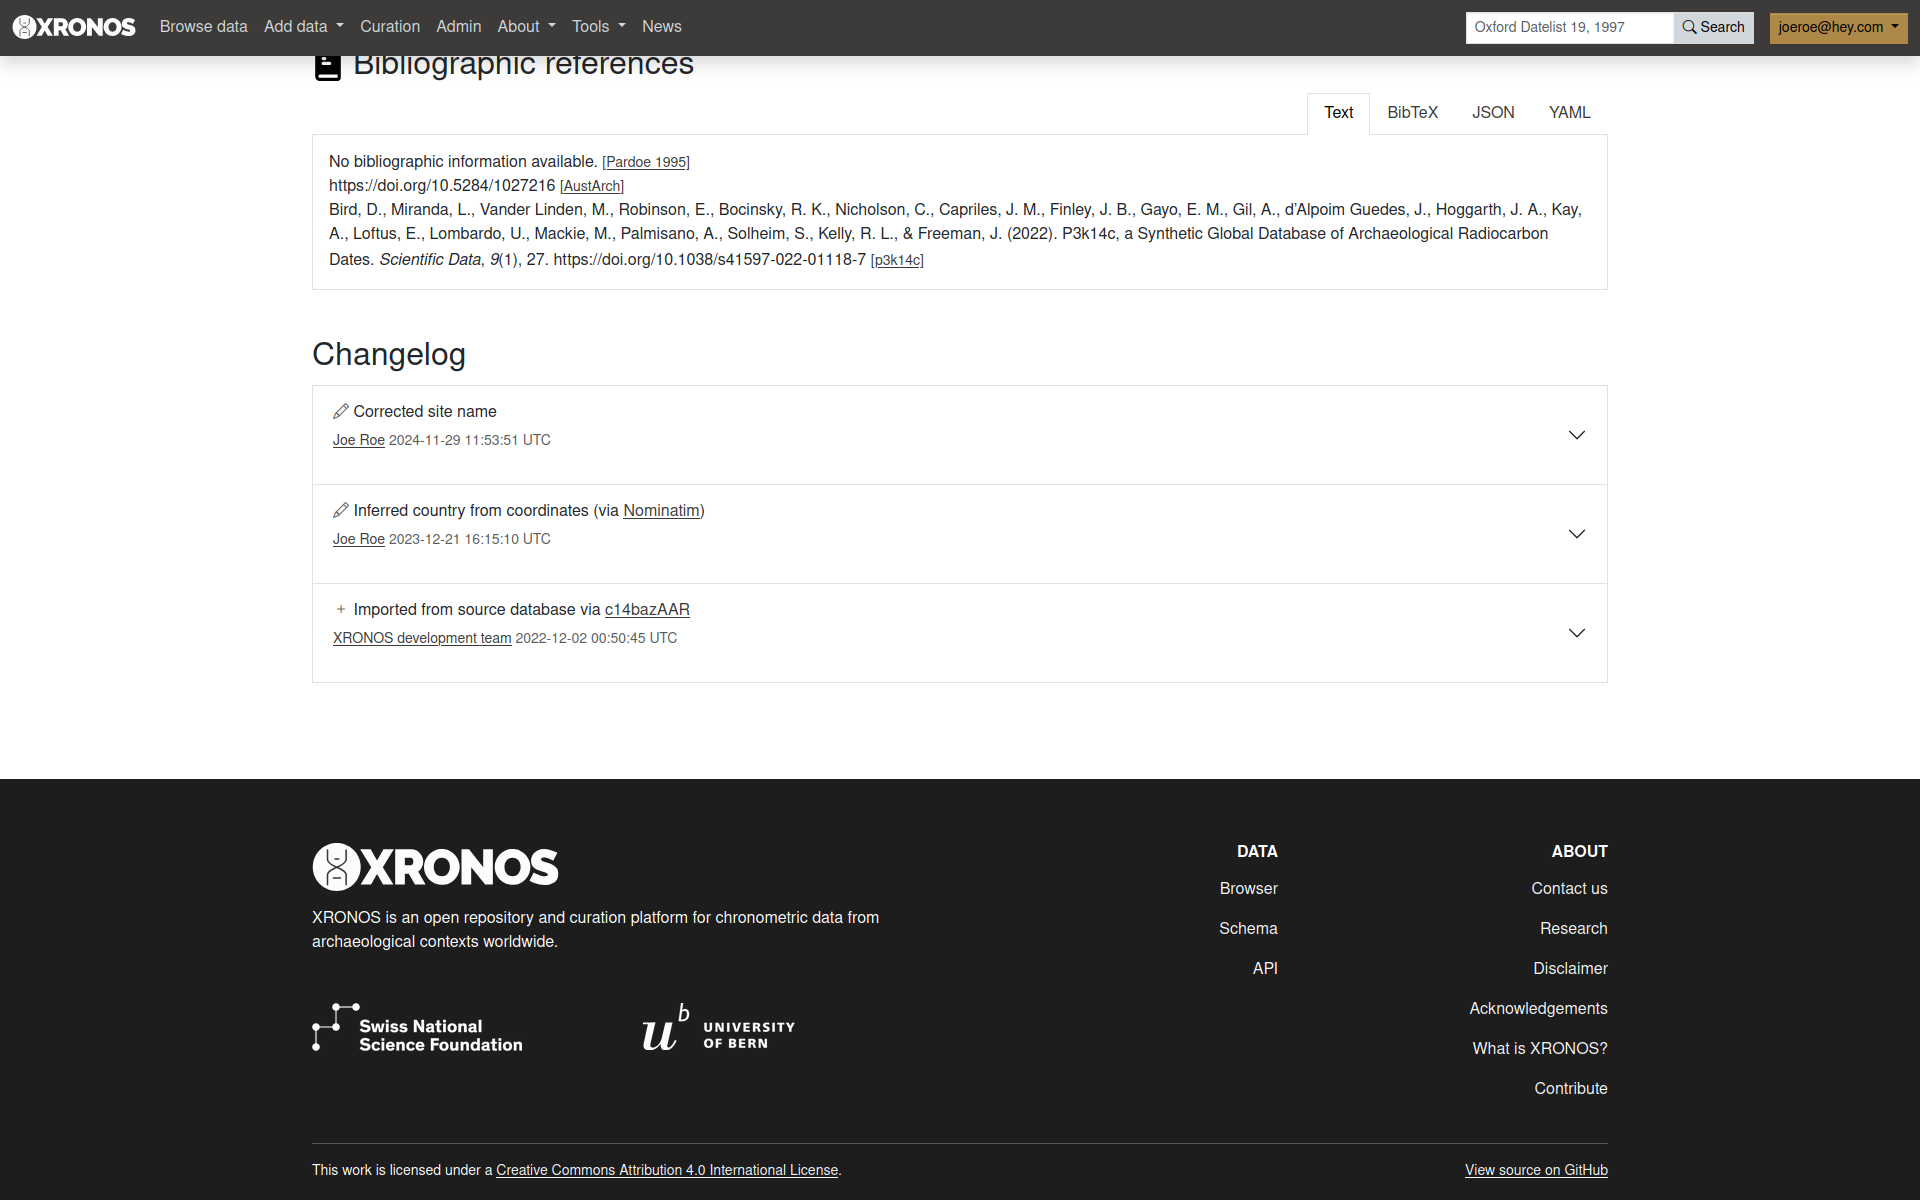
\includegraphics[keepaspectratio]{figures/xronos-ui-papertrail.png}}

}

\subcaption{\label{fig-ui-papertrail}Record change log}

\end{minipage}%
%
\begin{minipage}{0.50\linewidth}

\centering{

\pandocbounded{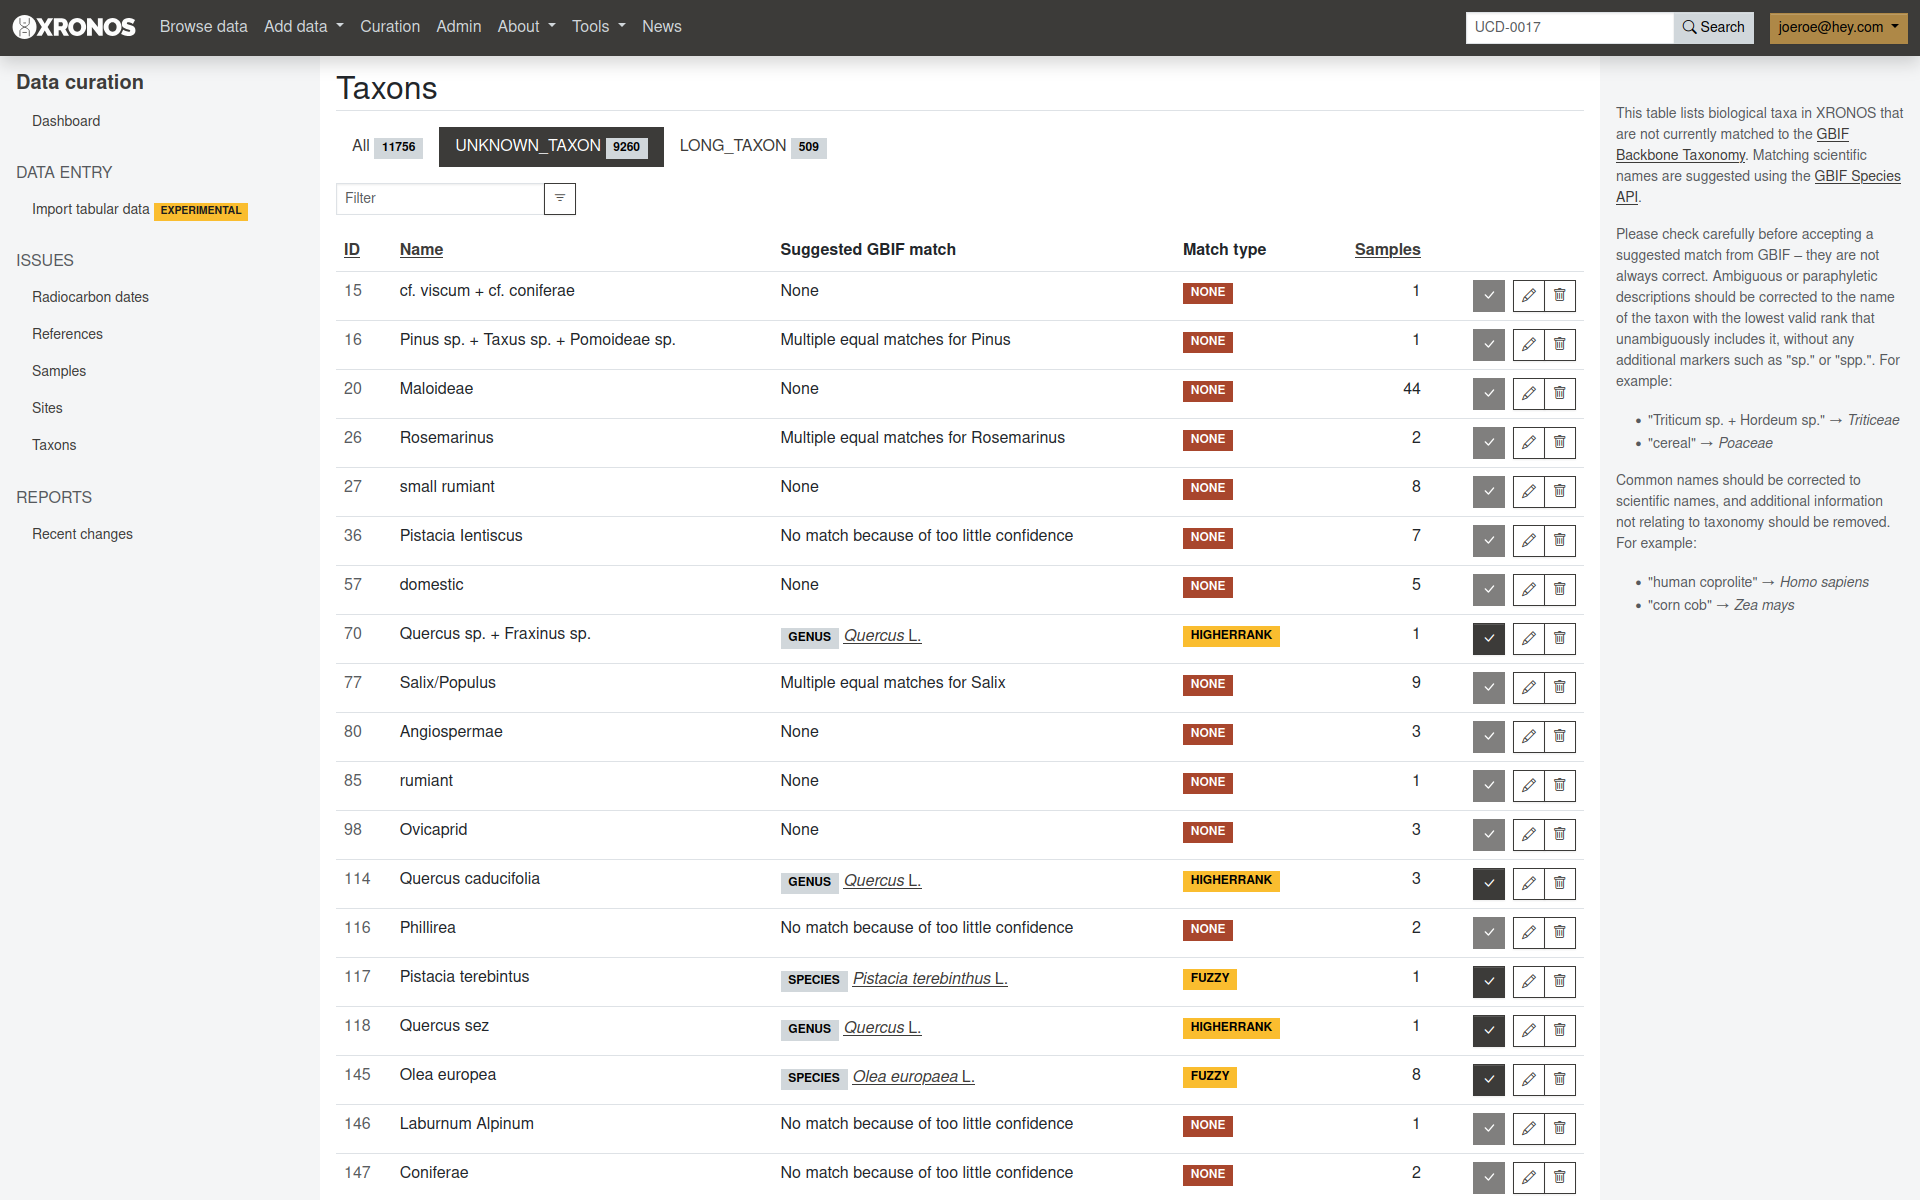
\includegraphics[keepaspectratio]{figures/xronos-ui-curation.png}}

}

\subcaption{\label{fig-ui-curation}Curation interface}

\end{minipage}%

\caption{\label{fig-ui}Views in the XRONOS web graphical user interface}

\end{figure}%

The graphical user interface (GUI) to XRONOS, accessed through a web
browser (e.g.~at \url{https://xronos.ch}), uses REST resources and
actions as the building blocks for various interfaces through which
users can browse, search, retrieve, and analyse chronometric data
(Figure~\ref{fig-ui}). Each action on each resource is represented by a
page, though not all of these are publicly accessible. The most import
of these are the `index' views, which list and summaries all instances
of a resource and support filtering and sorting; and `show' views (e.g.
Figure~\ref{fig-ui-show} for a site), which give a more comprehensive
information on an individual record along with visualisations, links to
related records, external linked open data resources, and a log of
changes made to the data since it was imported into XRONOS
(Figure~\ref{fig-ui-papertrail}). Pages representing REST resources
directly are supplemented by a number of synthetic interfaces, for
example the `data browser' (\url{https://xronos.ch/data},
Figure~\ref{fig-ui-data-browser}), which facilitates more complex
filtering, or the search interface (\url{https://xronos.ch/search}). The
GUI also includes several resources which are not part of XRONOS'
scientific data model, for example documentation pages, user profiles
and news articles; these are not exposed in the API.

Access to various `backstage' interfaces for creating, editing, and
deleting data, and monitoring data quality is managed using a user
permissions system. Currently only authorised users affiliated with the
XRONOS project can access these, but in the future we intend to support
open registration and expose editing interfaces to all authenticated
users. For this reason, there is no sharp division between a `public'
and `private' areas -- viewing/querying data and editing/curating data
share the same architecture and interface patterns.

The XRONOS API uses the same addresses as the web-based GUI (with the
exception of some of the synthetic interfaces mentioned above) but
responds with machine-readable data in JSON format, rather than a HTML
page. This response can be triggered by appending \texttt{.json} to the
address or by including a HTTP \texttt{content-format} header in the
request. Though users can make such requests manually and parse the data
with one of several off-the-shelf tools, the primary intended uses of
this interface is to provide access for 1) programmatic clients to
XRONOS and 2) other web services. The XRONOS R package (Hinz and Roe,
2024) is an example of a programmatic client; it uses the API to
facilitate direct querying and retrieval of data from XRONOS in the R
statistical programming language (R Core Team, 2024). Similar libraries
could be developed in other programming environments used for scientific
computing, such as Python or Haskell. The API also provides the
foundation for other web services to access XRONOS directly, to embed
chronological information in other contexts or otherwise make use of its
data resources.

An overarching principle of this software architecture is that all
interaction with XRONOS' data store, and as much of the data processing
and `business logic' of responding to REST requests as possible, is
directed through the same server-side routines. First and foremost, this
allows us to provide multiple interfaces (i.e.~the GUI and API, perhaps
more in the future) without duplicating these elements of our codebase.
It also improves accessibility for users accessing XRONOS through
devices with limited processing capability or through text-only
browsers. More broadly, avoiding reliance on client-side processing,
e.g.~with Javascript or Web Assembly (WASM)---which would be the other
option---allows us keep our client interfaces simple (in most cases
plain, semantic HTML pages and self-contained stylesheets) and
therefore, we hope, sustainable in the face of constantly-evolving
client-side technologies and standards. It does have the weakness that,
in practical terms, XRONOS is difficult to run and relies on the
continued existence of a maintained external server. We have however
tried to mitigate this by providing clearly-documented source code and
regular data dumps so that, if our instance of XRONOS disappears, or if
one simply does not want to use it, it is possible for others to host a
XRONOS server of their own. As the sustainability of scientific software
and data infrastructures is a pressing problem, in the future it may be
desirable to support further decentralisation through, for example, a
federated server-server model.

\section{Evaluation}\label{evaluation}

In this paper we have outlined the conceptual and technical
infrastructure developed during the initial, SNF-funded phases of
development on XRONOS in 2019 and 2021--2024. These include a
generalised data model for radiocarbon and typological dates, extendible
to other chronometric information, and associated contextual
information; an R- and Ruby-based pipeline for continuous ingestion of
data from a variety of sources; continuous, semi-automated data cleaning
protocols; a Ruby-on-Rails application providing a web-based frontend to
the data and a REST API for programmatic access; and an R package for
interfacing with the API. These systems are in production and publicly
accessible at \url{https://xronos.ch}.

At the current stage of implementation, we argue XRONOS provides a
framework for access to chronometric data that is more open, more
reliable, and more comprehensive than the previously available global
radiocarbon compilations. XRONOS blends aspects of the three existing
approaches (c14bazAAR, IntChron, and p3k14c; see Section
Section~\ref{sec-global-compilations}) to achieve the same aim of
providing access to the global radiocarbon data through a common
interface. Like c14bazAAR and IntChron, it is a `metadatabase' that
draws from existing data resources and maintains an explicit link to
them. But like p3k14c, it integrates these into a single database and
applies data curation processes to harmonise them and improve the
quality of the information. It has a wider scope than c14bazAAR or
IntChron, as it mirrors rather than directly retrieves the source data
(allowing us to use resources that aren't openly published), and does
not rely on the authors of these sources to implement a common
specification. It also goes beyond the functionality of p3k14c by
providing systems for the continuous ingestion and curation of new data
as it is published. With that said, we see the approaches followed by as
complementary rather than competing. A c14bazAAR parser for XRONOS is in
development (\url{https://github.com/ropensci/c14bazAAR/pull/150}), and
we also aim to provide an IntChron interface to XRONOS' data in the near
future. New data and corrections from p3k14c are incorporated into
XRONOS as they are released.

From 2025, development of XRONOS will continue within the framework of
`ESTER', an ERC-funded research project on estimation of prehistoric
population development from large, multiproxy datasets. Our immediate
development goals include the incorporation of dendrochronology into the
database, further refinement of our data curation pipelines, and the
public release of the editing interfaces.

Looking beyond the near term, we have endeavoured to create a
sustainable infrastructure that can be maintained by a wider scholarly
commons -- though we must acknowledge that this is a difficult problem,
and one that is as much organisational than technical. The source code
for all the software components of the system are available online (at
\url{https://github.com/xronos-ch}) under open licenses. The databases
of the instance at \url{https://xronos.ch} are also archived with Zenodo
(\emph{link omitted for blind review}). With these two resources we
reduce XRONOS' `bus factor'; if we are not able to continue operating
XRONOS, somebody else can fully recreate it. Equally importantly, we
enable the `right to fork' should others wish to take the software
and/or database in another direction. But aside from these extreme
scenarios, the long-term sustainability of XRONOS is contingent on the
existence of a community of scholars that use and contribute back to it.

\section{Acknowledgements}\label{acknowledgements}

The XRONOS project was carried under the direction of Albert Hafner.
Individual contributors to the XRONOS database to date include Chiara
Huwiler, Rivana Moser, Tomasz Chmielewski, and Stephanie Döppler. A
complete and up-to-date list of acknowledgements for the project can be
found at \url{https://xronos.ch/about/acknowledgements}.

\section{Funding Statement}\label{funding-statement}

This work was funded by the Swiss National Science Foundation
(\href{https://data.snf.ch/grants/grant/198153}{SNSF Project \#198152})
and the University of Bern (UniBE Initiator Grant 2019, Caroline Heitz,
Project `Time and Temporality').

\section{Data Accessibility
Statement}\label{data-accessibility-statement}

The data and R code used to produce our analysis of the state of the art
in radiocarbonc compilation, including all the figures presented here,
can be accessed via Zenodo at (\emph{link omitted for blind review,
included in submission materials})

The database and software described in this paper is open source and can
be accessed at \url{https://github.com/xronos-ch}.

\section*{References}\label{references}
\addcontentsline{toc}{section}{References}

\phantomsection\label{refs}
\begin{CSLReferences}{1}{0}
\bibitem[\citeproctext]{ref-Aitken1999}
Aitken, M.J., 1999. Science-{Based Dating} in {Archaeology}. Routledge,
London. \url{https://doi.org/10.4324/9781315836645}

\bibitem[\citeproctext]{ref-Al-Abyadh-Balghelam-Dalma-JebelEtAl}
Al-Abyadh-Balghelam-Dalma-Jebel, A., Dhanna-Marawah-Marawah, M.R., Yas,
R.G.-R.-S.B., n.d. {ADIAS Radiocarbon Archive}.

\bibitem[\citeproctext]{ref-Alcantara2021}
Alcántara, A., 2021. Entre tepalcates. {Hacia} una comprensi{ó}n
historiogr{á}fica de la dataci{ó}n arqueom{é}trica en la arqueolog{í}a
mexicana (1950-2020) (PhD thesis).
\url{https://doi.org/10.13140/RG.2.2.24447.74400/2}

\bibitem[\citeproctext]{ref-AlcantaraPedrozainpress}
Alcántara, A., Pedroza, I., in press. Latin {American Radiocarbon} on
the {Web Databases} and {Datasets}: {A Mexican} and {Brazilian
Perspectives}. Radiocarbon.

\bibitem[\citeproctext]{ref-AlvesEtAl2018}
Alves, E.Q., Macario, K., Ascough, P., Bronk Ramsey, C., 2018. The
{Worldwide Marine Radiocarbon Reservoir Effect}: {Definitions},
{Mechanisms}, and {Prospects}. Reviews of Geophysics 56, 278--305.
\url{https://doi.org/10.1002/2017RG000588}

\bibitem[\citeproctext]{ref-AndersonEtAl2010}
Anderson, D.G., Miller, D.S., Yerka, S.J., Gillam, J.C., Johanson, E.N.,
Anderson, D.T., Goodyear, A.C., Smallwood, A.M., 2010.
\href{https://www.jstor.org/stable/40914542}{{PIDBA} ({Paleoindian
Database} of the {Americas}) 2010: {Current Status} and {Findings}}.
Archaeology of Eastern North America 38, 63--89.

\bibitem[\citeproctext]{ref-ArnoldLibby1951}
Arnold, J.R., Libby, W.F., 1951. Radiocarbon {Dates}. Science 113,
111--120. \url{https://doi.org/10.1126/science.113.2927.111}

\bibitem[\citeproctext]{ref-BadaHelfman1975}
Bada, J.L., Helfman, P.M., 1975. Amino acid racemization dating of
fossil bones. World Archaeology 7, 160--173.
\url{https://doi.org/10.1080/00438243.1975.9979630}

\bibitem[\citeproctext]{ref-Pleiades}
Bagnall, R., Talbert, R.J.A., Tom, E., et al., 2006.
\href{https://pleiades.stoa.org/}{Pleiades: {A Community-Built
Gazetteer} and {Graph} of {Ancient Places}}.

\bibitem[\citeproctext]{ref-Baillie2014}
Baillie, M.G.L., 2014. Tree-ring {Dating} and {Archaeology}. Routledge,
London. \url{https://doi.org/10.4324/9781315748689}

\bibitem[\citeproctext]{ref-BANADORA}
Banque {Nationale} de {Donn{é}es} {Radiocarbone} ({BANADORA}), n.d.

\bibitem[\citeproctext]{ref-BarceloAlvarezEtAl2013}
Barceló Álvarez, J.A., Bogdanović, I., Capuzzo, G., 2013. New
developments of tecnological and archaeological data bases: {The}
example of radiocarbon dating, in: Arqueolog{í}a: {Actas} Del {Primer
Congreso Internacional} de {Buenas Pr{á}cticas} En {Patrimonio Mundial},
2013, {ISBN} 978-84-941030-9-4, p{á}gs. 733-749. JAS Arqueolog{í}a, pp.
733--749.

\bibitem[\citeproctext]{ref-Batist2023}
Batist, Z., 2023. Archaeological data work as continuous and
collaborative practice. \url{https://doi.org/10.5281/zenodo.8373390}

\bibitem[\citeproctext]{ref-BatistRoe2024}
Batist, Z., Roe, J., 2024. Open {Archaeology}, {Open Source}?
{Collaborative} practices in an emerging community of archaeological
software engineers. Internet Archaeol.
\url{https://doi.org/10.11141/ia.67.13}

\bibitem[\citeproctext]{ref-Bayliss2015}
Bayliss, A., 2015. Quality in {Bayesian} chronological models in
archaeology. World Archaeol. 47, 677--700.
\url{https://doi.org/10.1080/00438243.2015.1067640}

\bibitem[\citeproctext]{ref-Bednarik2020}
Bednarik, R.G., 2020. The use of weathering indices in rock art science
and archaeology. Rock Art Research: The Journal of the Australian Rock
Art Research Association (AURA) 29, 59--84.
\url{https://doi.org/10.3316/ielapa.275310392544915}

\bibitem[\citeproctext]{ref-Benedict2009}
Benedict, J.B., 2009. A {Review} of {Lichenometric Dating} and {Its
Applications} to {Archaeology}. American Antiquity 74, 143--172.
\url{https://doi.org/10.1017/S0002731600047545}

\bibitem[\citeproctext]{ref-Benz2010}
Benz, M., 2010. {PPND} -- {The Platform} for {Neolithic Radiocarbon
Dates}.

\bibitem[\citeproctext]{ref-BirdEtAl2024}
Bird, D., Bocinsky, K., Vander Linden, M., 2024.
\href{https://github.com/people3k/p3k14c}{p3k14c: P3k14C: A synthetic
global database of archaeological radiocarbon dates}.

\bibitem[\citeproctext]{ref-BirdEtAl2022}
Bird, D., Miranda, L., Vander Linden, M., Robinson, E., Bocinsky, R.K.,
Nicholson, C., Capriles, J.M., Finley, J.B., Gayo, E.M., Gil, A.,
d'Alpoim Guedes, J., Hoggarth, J.A., Kay, A., Loftus, E., Lombardo, U.,
Mackie, M., Palmisano, A., Solheim, S., Kelly, R.L., Freeman, J., 2022.
P3k14c, a synthetic global database of archaeological radiocarbon dates.
Scientific Data 9, 27. \url{https://doi.org/10.1038/s41597-022-01118-7}

\bibitem[\citeproctext]{ref-BohnerSchyle2004}
Böhner, U., Schyle, D., 2004. Radiocarbon {CONTEXT} database.

\bibitem[\citeproctext]{ref-Brogger1905}
Brøgger, W.C., 1905. Strandliniens beliggenhed under stenalderen i det
sydøstlige Norge. I kommission hos H. Aschehoug \& Company.

\bibitem[\citeproctext]{ref-BronkRamsey2009}
Bronk Ramsey, C., 2009. Bayesian {Analysis} of {Radiocarbon Dates}.
Radiocarbon 51, 337--360.
\url{https://doi.org/10.1017/S0033822200033865}

\bibitem[\citeproctext]{ref-BronkRamseyEtAl2019}
Bronk Ramsey, C., Blaauw, M., Kearney, R., Staff, R.A.S., 2019. The
importance of open access to chronological information: The {IntChron}
initiative. Radiocarbon 61, 1--11.
\url{https://doi.org/10.1017/RDC.2019.21}

\bibitem[\citeproctext]{ref-BronkRamseyEtAl2009}
Bronk Ramsey, C., Higham, T.F.G., Brock, F., Baker, D., Ditchfield, P.,
2009. Radiocarbon {Dates} from the {Oxford Ams System}: {Archaeometry
Da}TEList 33. Archaeometry 51, 323--349.
\url{https://doi.org/10.1111/j.1475-4754.2008.00457.x}

\bibitem[\citeproctext]{ref-BuckEtAl1991}
Buck, C.E., Kenworthy, J.B., Litton, C.D., Smith, A.F.M., 1991.
Combining archaeological and radiocarbon information: A {Bayesian}
approach to calibration. Antiquity 65, 808--821.
\url{https://doi.org/10.1017/S0003598X00080534}

\bibitem[\citeproctext]{ref-Buckland2014}
Buckland, P.I., 2014. {SEAD} - {The Strategic Environmental Archaeology
Database Inter-linking Multiproxy Environmental Data} with
{Archaeological Investigations} and {Ecology}, in: Verhagen, P., Earl,
G. (Eds.), Archaeology in the {Digital Era}: {Papers} from the 40th
{Annual Conference} of {Computer Applications} and {Quantitative
Methods} in {Archaeology} ({CAA}), {Southampton}, 26-29 {March} 2012.
Amsterdam University Press, pp. 320--331.
\url{https://doi.org/10.1515/9789048519590-035}

\bibitem[\citeproctext]{ref-CanhosEtAl2004}
Canhos, V.P., Souza, S. de, Giovanni, R.D., Canhos, D.A.L., 2004. Global
{Biodiversity Informatics}: Setting the scene for a "new world" of
ecological forecasting. Biodiversity Informatics 1.
\url{https://doi.org/10.17161/bi.v1i0.3}

\bibitem[\citeproctext]{ref-Capriles2023}
Capriles, J.M., 2023. The {Bolivian Radiocarbon Database}: {A
Countrywide Compilation} of {Radiocarbon Dates}. Journal of Open
Archaeology Data 11. \url{https://doi.org/10.5334/joad.104}

\bibitem[\citeproctext]{ref-CapuzzoEtAl2014}
Capuzzo, G., Boaretto, E., Barceló, J.A., 2014. {EUBAR}: {A Database} of
{14C Measurements} for the {European Bronze Age}. {A Bayesian Analysis}
of {14C-Dated Archaeological Contexts} from {Northern Italy} and
{Southern France}. Radiocarbon 56, 851--869.
\url{https://doi.org/10.2458/56.17453}

\bibitem[\citeproctext]{ref-IRDD}
Chapple, R.M., 2019. Catalogue of {Radiocarbon Determinations} \&
{Dendrochronology Dates} ({August} 2019 release).

\bibitem[\citeproctext]{ref-ChaputGajewski2016}
Chaput, M.A., Gajewski, K., 2016. Radiocarbon dates as estimates of
ancient human population size. Anthropocene 15, 3--12.
\url{https://doi.org/10.1016/j.ancene.2015.10.002}

\bibitem[\citeproctext]{ref-ClistEtAl2023}
Clist, B., Denbow, J., Lanfranchi, R., 2023. Using the radiocarbon dates
of {Central Africa} for studying long-term demographic trends of the
last 50,000 years: Potential and pitfalls. Azania: Archaeological
Research in Africa 58, 235--293.
\url{https://doi.org/10.1080/0067270X.2023.2215649}

\bibitem[\citeproctext]{ref-CochraneEtAl2021}
Cochrane, E.E., Rieth, T.M., Filimoehala, D., 2021. The first
quantitative assessment of radiocarbon chronologies for initial pottery
in {Island Southeast Asia} supports multi-directional {Neolithic}
dispersal. PLOS ONE 16, e0251407.
\url{https://doi.org/10.1371/journal.pone.0251407}

\bibitem[\citeproctext]{ref-CourtneyMustaphi2016}
Courtney Mustaphi, C., 2016. Radiocarbon dates from eastern {Africa} in
the {CARD2}.0 format. \url{https://doi.org/10.7910/DVN/NJLNRJ}

\bibitem[\citeproctext]{ref-Crema2024}
Crema, E.R., 2024. A {Bayesian} alternative for {Aoristic} analyses in
archaeology. \url{https://doi.org/10.31219/osf.io/98qkx}

\bibitem[\citeproctext]{ref-Crema2022}
Crema, E.R., 2022. Statistical {Inference} of {Prehistoric Demography}
from {Frequency Distributions} of {Radiocarbon Dates}: {A Review} and a
{Guide} for the {Perplexed}. J Archaeol Method Theory 29, 1387--1418.
\url{https://doi.org/10.1007/s10816-022-09559-5}

\bibitem[\citeproctext]{ref-CremaEtAl2024}
Crema, E.R., Bloxam, A., Stevens, C.J., Vander Linden, M., 2024.
Modelling diffusion of innovation curves using radiocarbon data. Journal
of Archaeological Science 165, 105962.
\url{https://doi.org/10.1016/j.jas.2024.105962}

\bibitem[\citeproctext]{ref-CremaEtAl2016}
Crema, E.R., Habu, J., Kobayashi, K., Madella, M., 2016. Summed
{Probability Distribution} of {14C Dates Suggests Regional Divergences}
in the {Population Dynamics} of the {Jomon Period} in {Eastern Japan}.
PLoS One 11, e0154809.
\url{https://doi.org/10.1371/journal.pone.0154809}

\bibitem[\citeproctext]{ref-dErricoEtAl2011}
d'Errico, F., Banks, W.E., Vanhaeren, M., Laroulandie, V., Langlais, M.,
2011. {PACEA Geo-Referenced Radiocarbon Database}. PaleoAnthropology
2011, 1--12.

\bibitem[\citeproctext]{ref-DanielsEtAl1953}
Daniels, F., Boyd, C.A., Saunders, D.F., 1953. Thermoluminescence as a
{Research Tool}. Science 117, 343--349.
\url{https://doi.org/10.1126/science.117.3040.343}

\bibitem[\citeproctext]{ref-deSaulieuEtAl2017}
de Saulieu, G., Oslisly, R., Nlend, P., Garcin, Y., Chevillotte, H.,
Kuete, N., 2017. Plateforme des datations arch{é}ologiques d'{Afrique
Centrale}. Version 2, 03.

\bibitem[\citeproctext]{ref-DeeEtAl2013}
Dee, M., Wengrow, D., Shortland, A., Stevenson, A., Brock, F., Girdland
Flink, L., Bronk Ramsey, C., 2013. An absolute chronology for early
{Egypt} using radiocarbon dating and {Bayesian} statistical modelling.
Proceedings of the Royal Society A: Mathematical, Physical and
Engineering Sciences 469, 20130395.
\url{https://doi.org/10.1098/rspa.2013.0395}

\bibitem[\citeproctext]{ref-DeeEtAl2012}
Dee, M.W., Rowland, J.M., Higham, T.F.G., Shortland, A.J., Brock, F.,
Harris, S.A., Ramsey, C.B., 2012. Synchronising radiocarbon dating and
the {Egyptian} historical chronology by improved sample selection.
Antiquity 86, 868--883. \url{https://doi.org/10.1017/S0003598X00047979}

\bibitem[\citeproctext]{ref-Diaz-RodriguezEtAl2023}
Díaz-Rodríguez, M., Nielsen, T.K., Maier, A., Riede, F., 2023. An
{Annotated Compilation} of {Chronometric Dates} for the {Middle-Upper
Palaeolithic Transition} (45-30 ka {BP}) in {Northern Iberia} ({Spain}).
Journal of Open Archaeology Data 11.
\url{https://doi.org/10.5334/joad.113}

\bibitem[\citeproctext]{ref-Douglass1929}
Douglass, A.E., 1929. The secret of the {Southwest} solved by talkative
tree rings. National Geographic 56, 737--770.

\bibitem[\citeproctext]{ref-DouglassEtAl2019}
Douglass, K., Hixon, S., Wright, H.T., Godfrey, L.R., Crowley, B.E.,
Manjakahery, B., Rasolondrainy, T., Crossland, Z., Radimilahy, C., 2019.
A critical review of radiocarbon dates clarifies the human settlement of
{Madagascar}. Quat. Sci. Rev. 221, 105878.
\url{https://doi.org/10.1016/j.quascirev.2019.105878}

\bibitem[\citeproctext]{ref-EverndenEtAl1965}
Evernden, J.F., Curtis, G.H., Bishop, W., Brace, C.L., Clark, J.D.,
Damon, P.E., Hay, R.L., Hopkins, D.M., Howell, F.C., Knopf, A., Kretzoi,
M., Leakey, L.S.B., Maude, H.E., Richards, J.R., Savage, D.E., Wright,
H.E., 1965. The {Potassium-Argon Dating} of {Late Cenozoic Rocks} in
{East Africa} and {Italy} {[}and {Comments} and {Reply}{]}. Current
Anthropology 6, 342--385. \url{https://doi.org/10.1086/200619}

\bibitem[\citeproctext]{ref-FlohrEtAl2016}
Flohr, P., Fleitmann, D., Matthews, R., Matthews, W., Black, S., 2016.
Evidence of resilience to past climate change in {Southwest Asia}:
{Early} farming communities and the 9.2 and 8.2 ka events. Quat. Sci.
Rev. 136, 23--39. \url{https://doi.org/10.1016/j.quascirev.2015.06.022}

\bibitem[\citeproctext]{ref-Ford1962}
Ford, J.A., 1962. A quantitative method for deriving cultural
chronology, Manuales técnicos. Pan American Union, Washington.

\bibitem[\citeproctext]{ref-GajewskiEtAl2011}
Gajewski, K., Munoz, S., Peros, M., Viau, A., Morlan, R., Betts, M.,
2011. The {Canadian Archaeological Radiocarbon Database} ({Card}):
{Archaeological 14C Dates} in {North America} and {Their
Paleoenvironmental Context}. Radiocarbon 53, 371--394.
\url{https://doi.org/10.1017/S0033822200056630}

\bibitem[\citeproctext]{ref-GarnettEtAl2023}
Garnett, M.H., Bryant, C.L., Freeman, S.P.H.T., Gulliver, P., Ascough,
P.L., 2023. A {DATABASE OF NERC RADIOCARBON MEASUREMENTS DETERMINED BY
ACCELERATOR MASS SPECTROMETRY}. Radiocarbon 1--4.
\url{https://doi.org/10.1017/RDC.2023.18}

\bibitem[\citeproctext]{ref-GayoEtAl2015}
Gayo, E.M., Latorre, C., Santoro, C.M., 2015. Timing of occupation and
regional settlement patterns revealed by time-series analyses of an
archaeological radiocarbon database for the {South-Central Andes}
(16{\(^\circ\)}--25{\(^\circ\)}{S}). Quaternary International,
Palaeodemography in {Southern South America} 356, 4--14.
\url{https://doi.org/10.1016/j.quaint.2014.09.076}

\bibitem[\citeproctext]{ref-GBIF2023}
GBIF Secretariat, 2023. {GBIF Backbone Taxonomy}.
\url{https://doi.org/10.15468/39OMEI}

\bibitem[\citeproctext]{ref-GillespieEtAl1984}
Gillespie, R., Gowlett, J.a.J., Hall, E.T., Hedges, R.E.M., 1984.
Radiocarbon {Measurement} by {Accelerator Mass Spectrometry}: {An Early
Selection} of {Dates}. Archaeometry 26, 15--20.
\url{https://doi.org/10.1111/j.1475-4754.1984.tb00313.x}

\bibitem[\citeproctext]{ref-GregoriodeSouza2020}
Gregorio de Souza, J., 2020. Rxpand: {Radiocarbon} dates for the spread
of farming and ceramics in tropical {South America}.

\bibitem[\citeproctext]{ref-GrossmannEtAl2023}
Großmann, R., Weinelt, M., Müller, J., 2023. Demographic dynamics
between 5500 and 3500 {calBP} (3550--1550 {BCE}) in selected study
regions of {Central Europe} and the role of regional climate influences.
PLOS ONE 18, e0291956.
\url{https://doi.org/10.1371/journal.pone.0291956}

\bibitem[\citeproctext]{ref-Grove2011}
Grove, M., 2011. A {Spatio-Temporal Kernel Method} for {Mapping Changes}
in {Prehistoric Land-Use Patterns}. Archaeometry 53, 1012--1030.
\url{https://doi.org/10.1111/j.1475-4754.2010.00578.x}

\bibitem[\citeproctext]{ref-HannahEtAl2022}
Hannah, E., Carlin, N., Griffiths, S., Gaydarska, B., Swan, R., Corns,
A., 2022. \href{https://www.jstor.org/stable/27198744}{Project
{Radiocarbon}}. Archaeology Ireland 36, 14--17.

\bibitem[\citeproctext]{ref-Harding1999}
Harding, A., 1999. Establishing {Archaeological Chronologies}, in:
Companion {Encyclopedia} of {Archaeology}. Routledge.

\bibitem[\citeproctext]{ref-Harris1979}
Harris, E.C., 1979. The laws of archaeological stratigraphy. World
Archaeology 11, 111--117.
\url{https://doi.org/10.1080/00438243.1979.9979753}

\bibitem[\citeproctext]{ref-HermankovaEtAl2021}
Heřmánková, P., Kaše, V., Sobotková, A., 2021. Inscriptions as data:
Digital epigraphy in macro-historical perspective. Journal of Digital
History 1, 99--141. \url{https://doi.org/10.1515/jdh-2021-1004}

\bibitem[\citeproctext]{ref-HighamEtAl2014}
Higham, T., Douka, K., Wood, R., Ramsey, C.B., Brock, F., Basell, L.,
Camps, M., Arrizabalaga, A., Baena, J., Barroso-Ruíz, C., Bergman, C.,
Boitard, C., Boscato, P., Caparrós, M., Conard, N.J., Draily, C.,
Froment, A., Galván, B., Gambassini, P., Garcia-Moreno, A., Grimaldi,
S., Haesaerts, P., Holt, B., Iriarte-Chiapusso, M.-J., Jelinek, A.,
Jordá Pardo, J.F., Maíllo-Fernández, J.-M., Marom, A., Maroto, J.,
Menéndez, M., Metz, L., Morin, E., Moroni, A., Negrino, F.,
Panagopoulou, E., Peresani, M., Pirson, S., de la Rasilla, M.,
Riel-Salvatore, J., Ronchitelli, A., Santamaria, D., Semal, P., Slimak,
L., Soler, J., Soler, N., Villaluenga, A., Pinhasi, R., Jacobi, R.,
2014. The timing and spatiotemporal patterning of {Neanderthal}
disappearance. Nature 512, 306--309.
\url{https://doi.org/10.1038/nature13621}

\bibitem[\citeproctext]{ref-RADON}
Hinz, M., Furholt, M., Müller, J., Raetzel-Fabian, D., Rinne, C.,
Sjögren, K.-G., Wotzka, H.-P., 2012. {RADON} - {Radiocarbon} dates
online 2012. {Central European} database of {14C} dates for the
{Neolithic} and {Early Bronze Age}. Jungsteinsite 14, 1--4.

\bibitem[\citeproctext]{ref-HinzRoe2024}
Hinz, M., Roe, J., 2024.
\href{https://github.com/xronos-ch/xronos.R}{Xronos: Client for the
'XRONOS' chronological database}.

\bibitem[\citeproctext]{ref-HoebeEtAl2023}
Hoebe, P.W., Peeters, J.H.M., Arnoldussen, S., 2023. Parsing prehistoric
patterns: {Prospects} and limitations of a big radiocarbon dataset for
understanding the impact of climate on {Late Palaeolithic} and
{Mesolithic} populations in northwest {Europe} (16--7.5~ka {calBP}).
Journal of Archaeological Science: Reports 49, 103944.
\url{https://doi.org/10.1016/j.jasrep.2023.103944}

\bibitem[\citeproctext]{ref-HoggarthEtAl2021}
Hoggarth, J.A., Ebert, C.E., Castelazo-Calva, V.E., 2021. {MesoRAD}: {A
New Radiocarbon Data Set} for {Archaeological Research} in
{Mesoamerica}. Journal of Open Archaeology Data 9, 10.
\url{https://doi.org/10.5334/joad.83}

\bibitem[\citeproctext]{ref-HuetEtAl2024}
Huet, T., Basílio, A.C., Carvalho, A.F., Cubas, M., Gibaja, J.F.,
López-Romero, E., Oms, F.X., Mazzucco, N., 2024. {NeoNet Atlantic}.
{Radiocarbon Dates} for the {Late Mesolithic}/{Early Neolithic
Transition} in the {Southern European Atlantic Coast} 12, 2.
\url{https://doi.org/10.5334/joad.120}

\bibitem[\citeproctext]{ref-HuetEtAl2022}
Huet, T., Cubas, M., Gibaja, J.F., Oms, F.X., Mazzucco, N., 2022.
{NeoNet Dataset}. {Radiocarbon Dates} for the {Late Mesolithic}/{Early
Neolithic Transition} in the {North Central-Western Mediterranean
Basin}. Journal of Open Archaeology Data 10, 3.
\url{https://doi.org/10/gpk67w}

\bibitem[\citeproctext]{ref-KatsianisEtAl2020}
Katsianis, M., Bevan, A., Styliaras, G., Maniatis, Y., 2020. An {Aegean
History} and {Archaeology Written} through {Radiocarbon Dates}. Journal
of Open Archaeology Data 8. \url{https://doi.org/10.5334/joad.65}

\bibitem[\citeproctext]{ref-KellyEtAl2022}
Kelly, R.L., Mackie, M.E., Robinson, E., Meyer, J., Berry, M.,
Boulanger, M., Codding, B.F., Freeman, J., Garland, C.J., Gingerich, J.,
Hard, R., Haug, J., Martindale, A., Meeks, S., Miller, M., Miller, S.,
Perttula, T., Railey, J.A., Reid, K., Scharlotta, I., Spangler, J.,
Thomas, D.H., Thompson, V., White, A., 2022. A {New Radiocarbon
Database} for the {Lower} 48 {States}. American Antiquity 87, 581--590.
\url{https://doi.org/10.1017/aaq.2021.157}

\bibitem[\citeproctext]{ref-KemmersMyrberg2011}
Kemmers, F., Myrberg, N., 2011. Rethinking numismatics. {The}
archaeology of coins. Archaeological Dialogues 18, 87--108.
\url{https://doi.org/10.1017/S1380203811000146}

\bibitem[\citeproctext]{ref-KimEtAl2021}
Kim, H., Lee, G.-A., Crema, E.R., 2021. Bayesian analyses question the
role of climate in {Chulmun} demography. Scientific Reports 11, 23797.
\url{https://doi.org/10.1038/s41598-021-03180-4}

\bibitem[\citeproctext]{ref-Kintigh2006}
Kintigh, K., 2006. The promise and challenge of archaeological data
integration. Am. Antiq. 71, 567--578.
\url{https://doi.org/10.1017/S0002731600039810}

\bibitem[\citeproctext]{ref-RADONB}
Kneisel, J., Hinz, M., Rinne, C., 2014. {RADON-B} -- {Radiocarbon} dates
online (version 2014). {Database} for {European 14C} dates for the
{Bronze} and {Early Iron Age}.

\bibitem[\citeproctext]{ref-Kra1989}
Kra, R., 1989. The {International Radiocarbon Data Base}: {A Progress
Report}. Radiocarbon 31, 1067--1075.
\url{https://doi.org/10.1017/S003382220001273X}

\bibitem[\citeproctext]{ref-Kra1988}
Kra, R., 1988. Updating the past: {The Establishment} of the
{International Radiocarbon Data Base}. American Antiquity 53, 118--125.
\url{https://doi.org/10.2307/281158}

\bibitem[\citeproctext]{ref-Kudo2018}
Kudo, Y., 2018. Approach for {Creating Database} of the {Radiocarbon
Dates Published} on the {Archaeological Research Reports} in {Japan}.
Bulletin of the National Museum of Japanese History 212, 251.

\bibitem[\citeproctext]{ref-KudoEtAl2023}
Kudo, Y., Sakamoto, M., Hakozaki, M., Stevens, C.J., Crema, E.R., 2023.
An {Archaeological Radiocarbon Database} of {Japan}. Journal of Open
Archaeology Data 11. \url{https://doi.org/10.5334/joad.115}

\bibitem[\citeproctext]{ref-KusumgarEtAl1963}
Kusumgar, S., Lal, D., Sarna, R.P., 1963. Tata {Institute Radiocarbon
Date List I}. Radiocarbon 5, 273--282.
\url{https://doi.org/10.1017/S0033822200036894}

\bibitem[\citeproctext]{ref-Lake2012}
Lake, M., 2012. Open archaeology. World Archaeology 44, 471--478.
\url{https://doi.org/10.1080/00438243.2012.748521}

\bibitem[\citeproctext]{ref-LawrenceEtAl2020}
Lawrence, C.R., Beem-Miller, J., Hoyt, A.M., Monroe, G., Sierra, C.A.,
Stoner, S., Heckman, K., Blankinship, J.C., Crow, S.E., McNicol, G.,
Trumbore, S., Levine, P.A., Vindušková, O., Todd-Brown, K., Rasmussen,
C., Hicks Pries, C.E., Schädel, C., McFarlane, K., Doetterl, S., Hatté,
C., He, Y., Treat, C., Harden, J.W., Torn, M.S., Estop-Aragonés, C.,
Asefaw Berhe, A., Keiluweit, M., Della Rosa Kuhnen, Á., Marin-Spiotta,
E., Plante, A.F., Thompson, A., Shi, Z., Schimel, J.P., Vaughn, L.J.S.,
von Fromm, S.F., Wagai, R., 2020. An open-source database for the
synthesis of soil radiocarbon data: {International Soil Radiocarbon
Database} ({ISRaD}) version 1.0. Earth System Science Data 12, 61--76.
\url{https://doi.org/10.5194/essd-12-61-2020}

\bibitem[\citeproctext]{ref-LevyEtAl2021}
Levy, E., Geeraerts, G., Pluquet, F., Piasetzky, E., Fantalkin, A.,
2021. Chronological networks in archaeology: {A} formalised scheme.
Journal of Archaeological Science 127, 105225.
\url{https://doi.org/10.1016/j.jas.2020.105225}

\bibitem[\citeproctext]{ref-Libby1955}
Libby, W.F., 1955. Radiocarbon {Dating}, Second. ed. University of
Chicago Press.

\bibitem[\citeproctext]{ref-LinnenluckeEtAl2023}
Linnenlucke, L., Bird, M.I., Petchey, F., Alliston, G., McNiven, I.J.,
David, B., Ulm, S., 2023. Assessing the {Reliability} of a {Small-Scale
Legacy Radiocarbon Dataset Using Chronometric Transparency Approaches}:
{Torres Strait Radiocarbon Database}. Journal of Open Archaeology Data
11. \url{https://doi.org/10.5334/joad.95}

\bibitem[\citeproctext]{ref-Lipo2020}
Lipo, C., 2020. A repository of radiocarbon data for {Rapa Nui}.

\bibitem[\citeproctext]{ref-LoftusEtAl2019}
Loftus, E., Mitchell, P.J., Ramsey, C.B., 2019. An archaeological
radiocarbon database for southern {Africa}. Antiquity 93, 870--885.
\url{https://doi.org/10.15184/aqy.2019.75}

\bibitem[\citeproctext]{ref-LucariniEtAl2020}
Lucarini, G., Wilkinson, T., Crema, E.R., Palombini, A., Bevan, A.,
Broodbank, C., 2020. The {MedAfriCarbon Radiocarbon Database} and {Web
Application}. {Archaeological Dynamics} in {Mediterranean Africa}, ca.
9600--700 {BC}. Journal of Open Archaeology Data 8.
\url{https://doi.org/10.5334/joad.60}

\bibitem[\citeproctext]{ref-Lucas2004}
Lucas, G., 2004. Beyond chronology, in: The {Archaeology} of {Time}.
Routledge.

\bibitem[\citeproctext]{ref-ManningEtAl2016}
Manning, K., Colledge, S., Crema, E., Shennan, S., Timpson, A., 2016.
The {Cultural Evolution} of {Neolithic Europe}. {EUROEVOL Dataset} 1:
{Sites}, {Phases} and {Radiocarbon Data}. Journal of Open Archaeology
Data 5, 275. \url{https://doi.org/10.5334/joad.40}

\bibitem[\citeproctext]{ref-MaromWolkowski2024}
Marom, N., Wolkowski, U., 2024. A note on predator-prey dynamics in
radiocarbon datasets. Peer Community Journal 4.
\url{https://doi.org/10.24072/pcjournal.395}

\bibitem[\citeproctext]{ref-Martinez-GrauEtAl2021}
Martínez-Grau, H., Morell-Rovira, B., Antolín, F., 2021. Radiocarbon
{Dates Associated} to {Neolithic Contexts} ({Ca}. 5900 -- 2000 {Cal BC})
from the {Northwestern Mediterranean Arch} to the {High Rhine Area}.
Journal of Open Archaeology Data 9.
\url{https://doi.org/10.5334/joad.72}

\bibitem[\citeproctext]{ref-McFadgenEtAl2000}
McFadgen, B., Higham, T., Sparks, R.J., 2000. New {Zealand} radiocarbon
database for archaeology. Archaeology in New Zealand 43, 297--300.

\bibitem[\citeproctext]{ref-MichczynskiEtAl1995}
Michczyński, A., Krzanowski, A., Pazdur, M.F., Ziołkowski, M.S., 1995. A
{Computer-Based Database} for {Radiocarbon Dates} of {Central Andean
Archaeology}. Radiocarbon 37, 337--343.
\url{https://doi.org/10.1017/S0033822200030812}

\bibitem[\citeproctext]{ref-Millard2014}
Millard, A.R., 2014. Conventions for reporting radiocarbon
determinations. Radiocarbon 56, 555--559.
\url{https://doi.org/10.2458/56.17455}

\bibitem[\citeproctext]{ref-Mischka2004}
Mischka, D., 2004. Aoristische Analyse in der Archäologie.
Archäologische Informationen 27, 233--243.
\url{https://doi.org/10.11588/ai.2004.2.12685}

\bibitem[\citeproctext]{ref-MoodyEtAl2021}
Moody, B., Dye, T., May, K., Wright, H., Buck, C., 2021. Digital
chronological data reuse in archaeology: {Three} case studies with
varying purposes and perspectives. Journal of Archaeological Science:
Reports 40, 103188. \url{https://doi.org/10.1016/j.jasrep.2021.103188}

\bibitem[\citeproctext]{ref-NdeyeEtAl2022}
Ndeye, M., Athie, A.H., Kébé, D., Sène, M., 2022. {IFAN CH}.{DIOP
RADIOCARBON LABORATORY MEASUREMENTS II}. Radiocarbon 64, 397--414.
\url{https://doi.org/10.1017/RDC.2022.8}

\bibitem[\citeproctext]{ref-NelsonWade2015}
Nelson, A.J., Wade, A.D., 2015. Impact: {Development} of a {Radiological
Mummy Database}. The Anatomical Record 298, 941--948.
\url{https://doi.org/10.1002/ar.23130}

\bibitem[\citeproctext]{ref-OpenKnowledgeFoundation}
Open Knowledge Foundation, n.d. The {Open Definition}: {Defining Open}
in {Open Data}, {Open Content} and {Open Knowledge} {[}WWW Document{]}.
URL \url{https://opendefinition.org/} (accessed 11.25.2024).

\bibitem[\citeproctext]{ref-PalmisanoEtAl2022}
Palmisano, A., Bevan, A., Kabelindde, A., Roberts, N., Shennan, S.,
2022a. {AIDA}: {Archive} of {Italian} radiocarbon {DAtes}.

\bibitem[\citeproctext]{ref-PalmisanoEtAl2022a}
Palmisano, A., Bevan, A., Lawrence, D., Shennan, S., 2022b. The {NERD
Dataset}: {Near East Radiocarbon Dates} between 15,000 and 1,500 cal.
Yr. {BP} 10, 2. \url{https://doi.org/10.5334/joad.90}

\bibitem[\citeproctext]{ref-PalmisanoEtAl2017}
Palmisano, A., Bevan, A., Shennan, S., 2017. Data and code for
demographic trends in the paper "{Human} responses and non-responses to
climatic variations during the {Last Glacial-Interglacial} transition in
the eastern {Mediterranean}".
\url{https://doi.org/10.14324/000.ds.1570274}

\bibitem[\citeproctext]{ref-Pardo-GordoEtAl2023}
Pardo-Gordó, S., Vidal-Matutano, P., González-Marrero, M. del C.,
Chávez-Álvarez, M.E., 2023. The {14Canarias} web application. {An}
interactive radiocarbon database for the {Canary Islands}. Journal of
Open Archaeology Data 11. \url{https://doi.org/10.5334/joad.105}

\bibitem[\citeproctext]{ref-Perrin2019}
Perrin, T., 2019. \href{https://www.jstor.org/stable/26910790}{{BDA}:
Une {Base} de {Donn{é}es Arch{é}ologique} collaborative en ligne}.
Bulletin de la Soci{é}t{é} pr{é}historique fran{ç}aise 116, 159--162.

\bibitem[\citeproctext]{ref-PetcheyEtAl2022}
Petchey, F., Bickler, S., Hughes, L., Bunbury, M., 2022. The
{Aotearoa}/{New Zealand Radiocarbon Database Upgrade}. Archaeology in
New Zealand 65, 32--40.

\bibitem[\citeproctext]{ref-Petrie1899}
Petrie, W.M.F., 1899. Sequences in {Prehistoric Remains}. The Journal of
the Anthropological Institute of Great Britain and Ireland 29, 295--301.
\url{https://doi.org/10.2307/2843012}

\bibitem[\citeproctext]{ref-PettittEtAl2003}
Pettitt, P.B., Davies, W., Gamble, C.S., Richards, M.B., 2003.
Palaeolithic radiocarbon chronology: Quantifying our confidence beyond
two half-lives. J. Archaeol. Sci. 30, 1685--1693.
\url{https://doi.org/10.1016/S0305-4403(03)00070-0}

\bibitem[\citeproctext]{ref-PlompEtAl2022}
Plomp, E., Stantis, C., James, H.F., Cheung, C., Snoeck, C., Kootker,
L., Kharobi, A., Borges, C., Moreiras Reynaga, D.K., Pospieszny, Ł.,
Fulminante, F., Stevens, R., Alaica, A.K., Becker, A., de Rochefort, X.,
Salesse, K., 2022. The {IsoArcH} initiative: {Working} towards an open
and collaborative isotope data culture in bioarchaeology. Data in Brief
45, 108595. \url{https://doi.org/10.1016/j.dib.2022.108595}

\bibitem[\citeproctext]{ref-PratesEtAl2020}
Prates, L., Politis, G.G., Perez, S.I., 2020. Rapid radiation of humans
in {South America} after the last glacial maximum: {A} radiocarbon-based
study. PLOS ONE 15, e0236023.
\url{https://doi.org/10.1371/journal.pone.0236023}

\bibitem[\citeproctext]{ref-R2024}
R Core Team, 2024. \href{https://www.R-project.org/}{R: A language and
environment for statistical computing}. R Foundation for Statistical
Computing, Vienna, Austria.

\bibitem[\citeproctext]{ref-RabinowitzEtAl2016}
Rabinowitz, A., Shaw, R., Buchanan, S., Golden, P., Kansa, E., 2016.
Making {Sense} of the {Ways We Make Sense} of the {Past}: {The Periodo
Project}. Bulletin of the Institute of Classical Studies 59, 42--55.
\url{https://doi.org/10.1111/j.2041-5370.2016.12037.x}

\bibitem[\citeproctext]{ref-Rademaker2024}
Rademaker, K., 2024. Updated {Peru} archaeological radiocarbon database,
20,000--7000 {14C BP}. Quaternary International.
\url{https://doi.org/10.1016/j.quaint.2024.01.012}

\bibitem[\citeproctext]{ref-RademakerEtAl2013}
Rademaker, K., Bromley, G.R.M., Sandweiss, D.H., 2013. Peru
archaeological radiocarbon database, 13,000--7000 {14C B}.{P}.
Quaternary International, A {Late Pleistocene}/early {Holocene}
archaeological {14C} database for {Central} and {South America}:
Palaeoenvironmental contexts and demographic interpretations 301,
34--45. \url{https://doi.org/10.1016/j.quaint.2012.08.2052}

\bibitem[\citeproctext]{ref-RadiocarbonLabList}
Radiocarbon, 2024. Radiocarbon {Lab Information} {[}WWW Document{]}. URL
\url{https://radiocarbon.webhost.uits.arizona.edu/laboratories}
(accessed 11.25.2024).

\bibitem[\citeproctext]{ref-Raetzel-Fabian1999}
Raetzel-Fabian, D., 1999. Editorial. Jungsteinsite.

\bibitem[\citeproctext]{ref-RamseyEtAl2010}
Ramsey, C.B., Dee, M.W., Rowland, J.M., Higham, T.F.G., Harris, S.A.,
Brock, F., Quiles, A., Wild, E.M., Marcus, E.S., Shortland, A.J., 2010.
Radiocarbon-{Based Chronology} for {Dynastic Egypt}. Science 328,
1554--1557. \url{https://doi.org/10.1126/science.1189395}

\bibitem[\citeproctext]{ref-ReingruberThissen2017}
Reingruber, A., Thissen, L., 2017. The {14SEA Project}: {A 14C} database
for {Southeast Europe} and {Anatolia} (10,000--3000 {calBC}).

\bibitem[\citeproctext]{ref-ReingruberThissen2009}
Reingruber, A., Thissen, L., 2009. Depending on {14C Data}:
{Chronological Frameworks} in the {Neolithic} and {Chalcolithic} of
{Southeastern Europe}. Radiocarbon 51, 751--770.
\url{https://doi.org/10.1017/S0033822200056071}

\bibitem[\citeproctext]{ref-ReingruberThissen2005}
Reingruber, A., Thissen, L., 2005. {14C} database for the {Aegean}
catchment ({Eastern Greece}, southern {Balkans} and western {Turkey})
10,000--5500 cal {BC}, in: Lichter, C. (Ed.), How {Did Farming Reach
Europe}?, Byzas. Ege Yayinlar, Istanbul, pp. 295--327.

\bibitem[\citeproctext]{ref-ReiterEtAl2024}
Reiter, S.S., Staniuk, R., Kolář, J., Bulatović, J., Rose, H.A.,
Ryabogina, N.E., Speciale, C., Schjerven, N., Paulsson, B.S., Lee,
V.Y.K., Canteri, E., Revill, A., Dahlberg, F., Sabatini, S., Frei, K.M.,
Racimo, F., Ivanova-Bieg, M., Traylor, W., Kate, E.J., Derenne, E.,
Frank, L., Woodbridge, J., Fyfe, R., Shennan, S., Kristiansen, K.,
Thomas, M.G., Timpson, A., 2024. The BIAD standards: Recommendations for
archaeological data publication and insights from the big
interdisciplinary archaeological database. Open Archaeology 10,
20240015. \url{https://doi.org/doi:10.1515/opar-2024-0015}

\bibitem[\citeproctext]{ref-RichterEtAl2017}
Richter, T., Arranz-Otaegui, A., Yeomans, L., Boaretto, E., 2017. High
{Resolution AMS Dates} from {Shubayqa} 1, northeast {Jordan Reveal
Complex Origins} of {Late Epipalaeolithic Natufian} in the {Levant}.
Sci. Rep. 7, 17025. \url{https://doi.org/10.1038/s41598-017-17096-5}

\bibitem[\citeproctext]{ref-RADONB2024}
Rinne, C., Kneisel, J., Hinz, M., Furholt, M., Krischke, N., Müller, J.,
Raetzel-Fabian, D., Rodens, M., Sjögren, K.-G., Vandkilde, H., Wotzka,
H.-P., 2024. Rado.{NB}.

\bibitem[\citeproctext]{ref-Riris2021}
Riris, P., 2021. Carribean-{14C}: {A} compilation of 2147 anthropogenic
radiocarbon ({14C}) dates for the {Caribbean} region from 504 sites
across 57 islands.

\bibitem[\citeproctext]{ref-RirisEtAl2024}
Riris, P., Silva, F., Crema, E., Palmisano, A., Robinson, E., Siegel,
P.E., French, J.C., Jørgensen, E.K., Maezumi, S.Y., Solheim, S., Bates,
J., Davies, B., Oh, Y., Ren, X., 2024. Frequent disturbances enhanced
the resilience of past human populations. Nature 1--6.
\url{https://doi.org/10.1038/s41586-024-07354-8}

\bibitem[\citeproctext]{ref-Roalkvam2023}
Roalkvam, I., 2023. Shoredate: {An R} package for shoreline dating
coastal {Stone Age} sites. Journal of Open Source Software 8, 5337.
\url{https://doi.org/10.21105/joss.05337}

\bibitem[\citeproctext]{ref-Roe2024}
Roe, J., 2024. \href{https://github.com/joeroe/rintchron}{Rintchron:
Interface to IntChron}.

\bibitem[\citeproctext]{ref-SchmidEtAl2019}
Schmid, C., Seidensticker, D., Hinz, M., 2019. {c14bazAAR}: An r package
for downloading and preparing C14 dates from different source databases.
{Journal of Open Source Software} 4, 1914.
\url{https://doi.org/10.21105/joss.01914}

\bibitem[\citeproctext]{ref-SeidenstickerSchmid2021}
Seidensticker, D., Schmid, C., 2021. Dirkseidensticker/{aDRAC}: V2.0
{Pikunda}. \url{https://doi.org/10.5281/zenodo.4530717}

\bibitem[\citeproctext]{ref-SilvaSteele2014}
Silva, F., Steele, J., 2014. New methods for reconstructing geographical
effects on dispersal rates and routes from large-scale radiocarbon
databases. Journal of Archaeological Science 52, 609--620.
\url{https://doi.org/10.1016/j.jas.2014.04.021}

\bibitem[\citeproctext]{ref-Suess1967}
Suess, H.E., 1967.
\href{https://www.osti.gov/etdeweb/biblio/20895312}{Bristlecone pine
calibration of the radiocarbon time scale from 4100 {B}.{C}. To 1500
{B}.{C}}.

\bibitem[\citeproctext]{ref-TanindiErdogu2005}
Tanindi, O., Erdoğu, B., 2005. Recording the past: Towards an inventory
of the archaeological sites of {Turkey}. Conservation and Management of
Archaeological Sites 7, 125--130.
\url{https://doi.org/10.1179/135050305793137468}

\bibitem[\citeproctext]{ref-TenopirEtAl2011}
Tenopir, C., Allard, S., Douglass, K., Aydinoglu, A.U., Wu, L., Read,
E., Manoff, M., Frame, M., 2011. Data {Sharing} by {Scientists}:
{Practices} and {Perceptions}. PLOS ONE 6, e21101.
\url{https://doi.org/10.1371/journal.pone.0021101}

\bibitem[\citeproctext]{ref-Thomsen1836}
Thomsen, C.J., 1836. Ledetrad til {Nordiske Oldkindighed}. Copenhagen.

\bibitem[\citeproctext]{ref-UriarteGonzalezEtAl2017}
Uriarte González, A., Fernández Freire, C., Fraguas Bravo, A., Castañeda
Clemente, N., Capdevila Montes, E., Salas Tovar, E., Gilman, A., Bosque
González, I. del, Vicent García, J.M., 2017. {IDEArq-C14: Una
Infraestructura de Datos Espaciales para la cronolog{í}a
radiocarb{ó}nica de la Prehistoria Reciente ib{é}rica}.
\url{https://doi.org/10.13039/501100003329}

\bibitem[\citeproctext]{ref-VanStrydonckDeRoock}
Van Strydonck, M., De Roock, E., n.d. Radiocarbon and stable isotope
measurements. Royal Institute for Cultural Heritage.

\bibitem[\citeproctext]{ref-VerborghEtAl2015}
Verborgh, R., van Hooland, S., Cope, A.S., Chan, S., Mannens, E., Van de
Walle, R., 2015. The fallacy of the multi-{API} culture: {Conceptual}
and practical benefits of {Representational State Transfer} ({REST}).
Journal of Documentation 71, 233--252.
\url{https://doi.org/10.1108/JD-07-2013-0098}

\bibitem[\citeproctext]{ref-Vermeersch2024}
Vermeersch, P.M., 2024. Radiocarbon {Palaeolithic Europe Database}.

\bibitem[\citeproctext]{ref-Vermeersch2020}
Vermeersch, P.M., 2020. Radiocarbon {Palaeolithic Europe} database: {A}
regularly updated dataset of the radiometric data regarding the
{Palaeolithic} of {Europe}, {Siberia} included. Data Brief 31, 105793.
\url{https://doi.org/10.1016/j.dib.2020.105793}

\bibitem[\citeproctext]{ref-Voorburg2012}
Voorburg, R., 2012. Archaeological {Atlas} of {Antiquity} - {Vici}.org
{[}WWW Document{]}. URL \url{https://vici.org/} (accessed 11.25.2024).

\bibitem[\citeproctext]{ref-WangEtAl2014}
Wang, C., Lu, H., Zhang, J., Gu, Z., He, K., 2014. Prehistoric
demographic fluctuations in {China} inferred from radiocarbon data and
their linkage with climate change over the past 50,000 years. Quaternary
Science Reviews 98, 45--59.
\url{https://doi.org/10.1016/j.quascirev.2014.05.015}

\bibitem[\citeproctext]{ref-Weninger2022}
Weninger, B., 2022. {CalPal}.
\url{https://doi.org/10.5281/ZENODO.7215741}

\bibitem[\citeproctext]{ref-Whitley2012}
Whitley, D.S., 2012. In {Suspect Terrain}: {Dating Rock Engravings}, in:
A {Companion} to {Rock Art}. John Wiley \& Sons, Ltd, pp. 605--624.
\url{https://doi.org/10.1002/9781118253892.ch34}

\bibitem[\citeproctext]{ref-WilliamsSmith2013}
Williams, A.N., Smith, M., 2013.
\href{https://www.jstor.org/stable/23621983}{{AustArch3}: {A} database
of 14 {C} and luminescence ages from archaeological sites in southern
{Australia}}. Australian Archaeology 102--102.

\bibitem[\citeproctext]{ref-WilliamsSmith2012}
Williams, A.N., Smith, M.A., 2012.
\href{https://www.jstor.org/stable/23621556}{{AustArch2}: {A} database
of 14 {C} and luminescence ages from archaeological sites in the {Top
End}}. Australian Archaeology 146--146.

\bibitem[\citeproctext]{ref-WilliamsEtAl2008}
Williams, A.N., Smith, M.A., Turney, C.S.M., Cupper, M.L., 2008.
\href{https://www.jstor.org/stable/20839288}{{AustArch1}: {A Database}
of {\(^{14}\)}{C} and {Luminescence Ages} from {Archaeological Sites} in
the {Australian Arid Zone}}. Australian Archaeology 99--99.

\bibitem[\citeproctext]{ref-WilliamsEtAl2014}
Williams, A., Ulm, S., Smith, M., Reid, J., 2014. {AustArch}: {A
Database} of {14C} and {Non-14C Ages} from {Archaeological Sites} in
{Australia} - {Composition}, {Compilation} and {Review} ({Data Paper}).
Internet Archaeology. \url{https://doi.org/10.11141/ia.36.6}

\bibitem[\citeproctext]{ref-WilliamsEtAl2018}
Williams, J.W., Grimm, E.C., Blois, J.L., Charles, D.F., Davis, E.B.,
Goring, S.J., Graham, R.W., Smith, A.J., Anderson, M., Arroyo-Cabrales,
J., Ashworth, A.C., Betancourt, J.L., Bills, B.W., Booth, R.K.,
Buckland, P.I., Curry, B.B., Giesecke, T., Jackson, S.T., Latorre, C.,
Nichols, J., Purdum, T., Roth, R.E., Stryker, M., Takahara, H., 2018.
The {Neotoma Paleoecology Database}, a multiproxy, international,
community-curated data resource. Quaternary Research 89, 156--177.
\url{https://doi.org/10.1017/qua.2017.105}

\bibitem[\citeproctext]{ref-Worsaae1843}
Worsaae, J.J.A., 1843. Danmarks Oldtid oplyst ved Oldsager og Gravhøie.
Selskabet for Trykkefrihedens rette Brug, Copenhagen.

\end{CSLReferences}




\end{document}
